\section{ИССЛЕДОВАНИЕ РАБОТЫ ЛОГИЧЕСКИХ ЭЛЕМЕНТОВ}

\subsection{Элемент НЕ}

\begin{figure}[H]
	\centering
	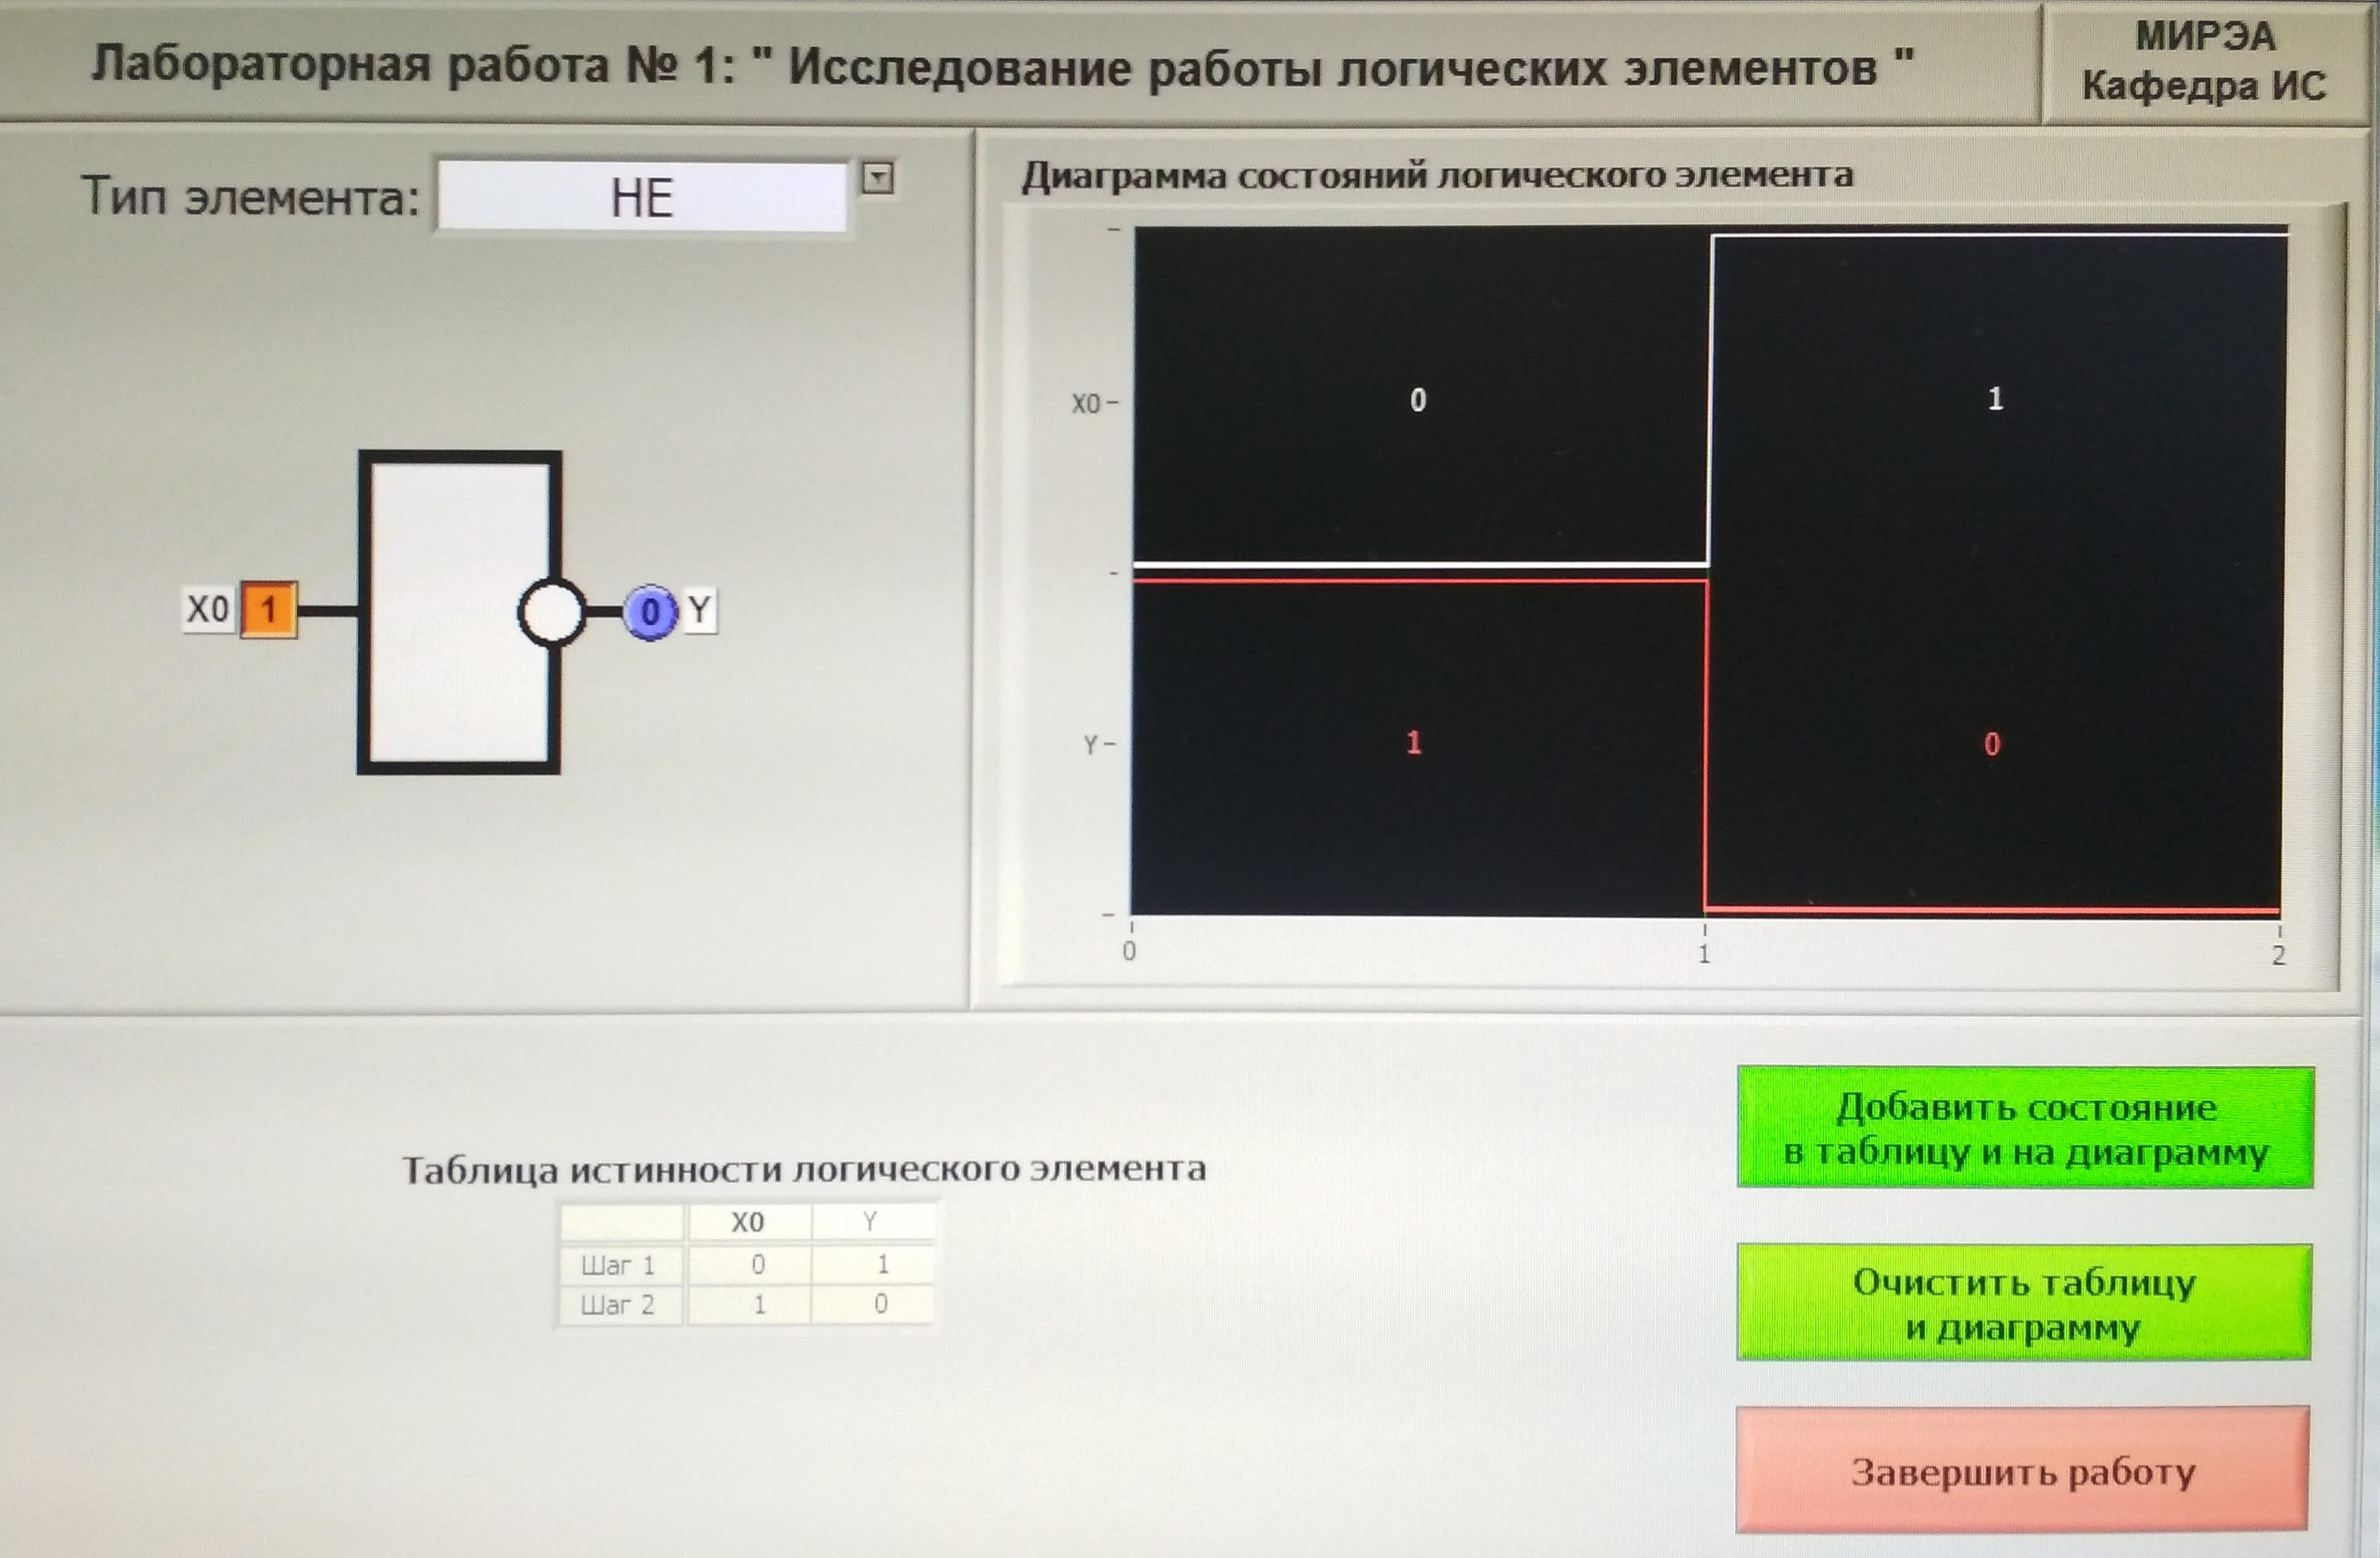
\includegraphics[width=0.85\linewidth]{imgs/1/not}
	\caption{Результат схемы НЕ}
	\label{fig:1_not}
\end{figure}

\begin{figure}[H]
	\centering
	\begin{minipage}{.45\textwidth}
		\centering
		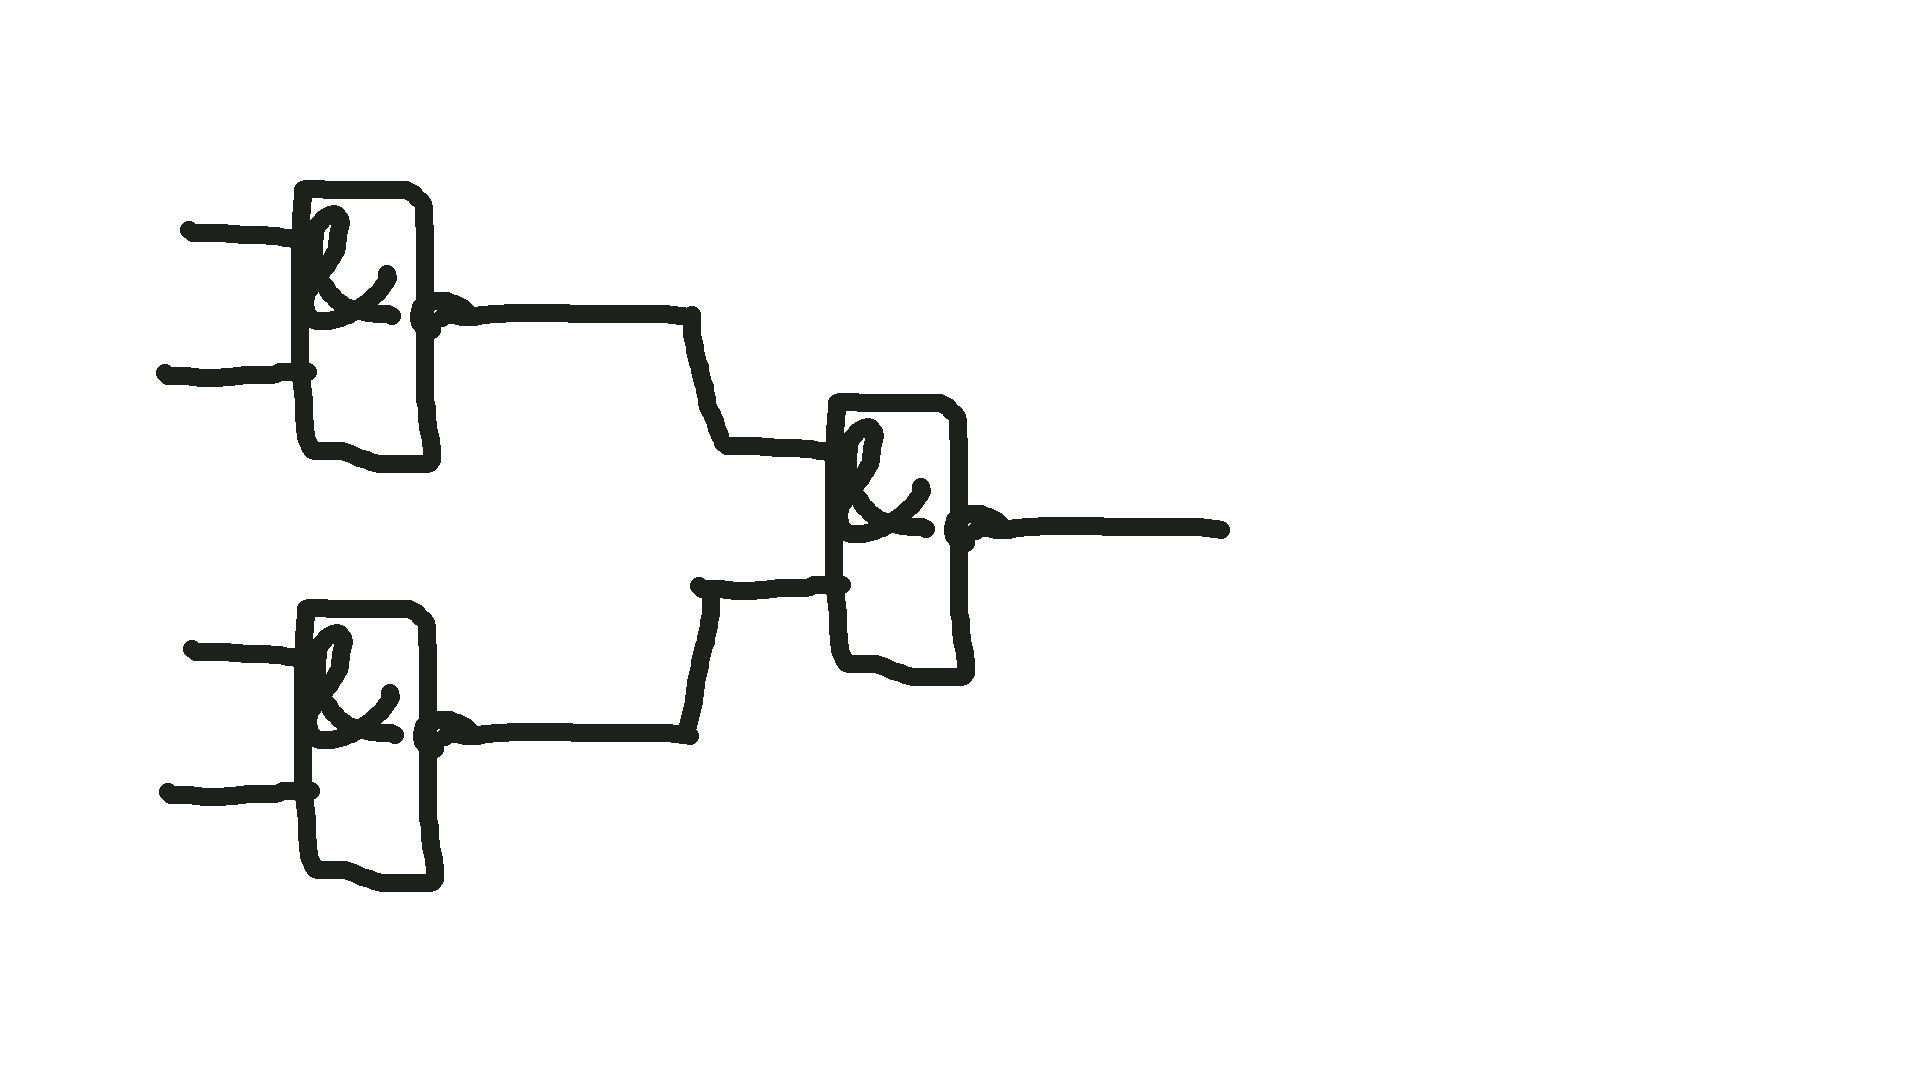
\includegraphics[width=0.85\linewidth]{imgs/1/not_and}
	\end{minipage}
	\begin{minipage}{.45\textwidth}
		\centering
		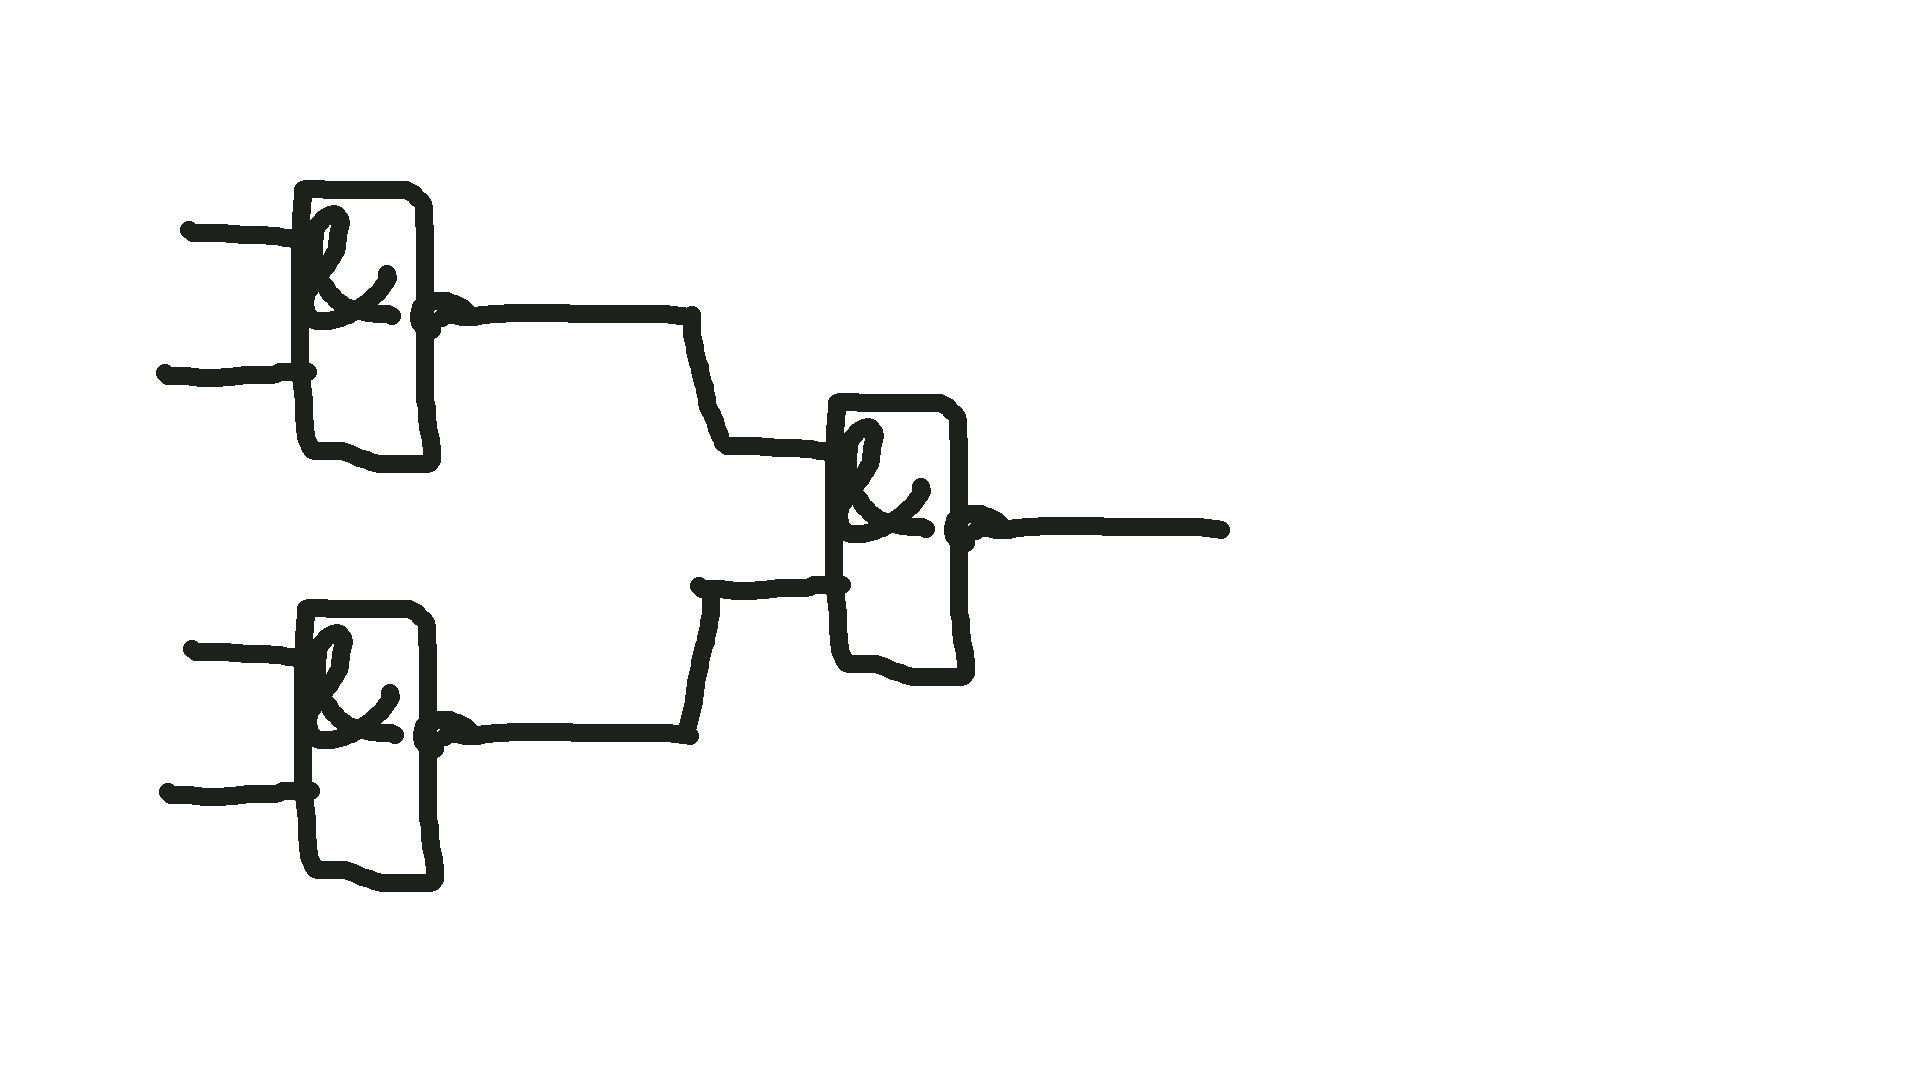
\includegraphics[width=0.85\linewidth]{imgs/1/not_or}
	\end{minipage}
	\caption{Реализация элемента НЕ в базисах 2И-НЕ и 2ИЛИ-НЕ}
\end{figure}

\subsection{Элемент И}

\begin{figure}[H]
	\centering
	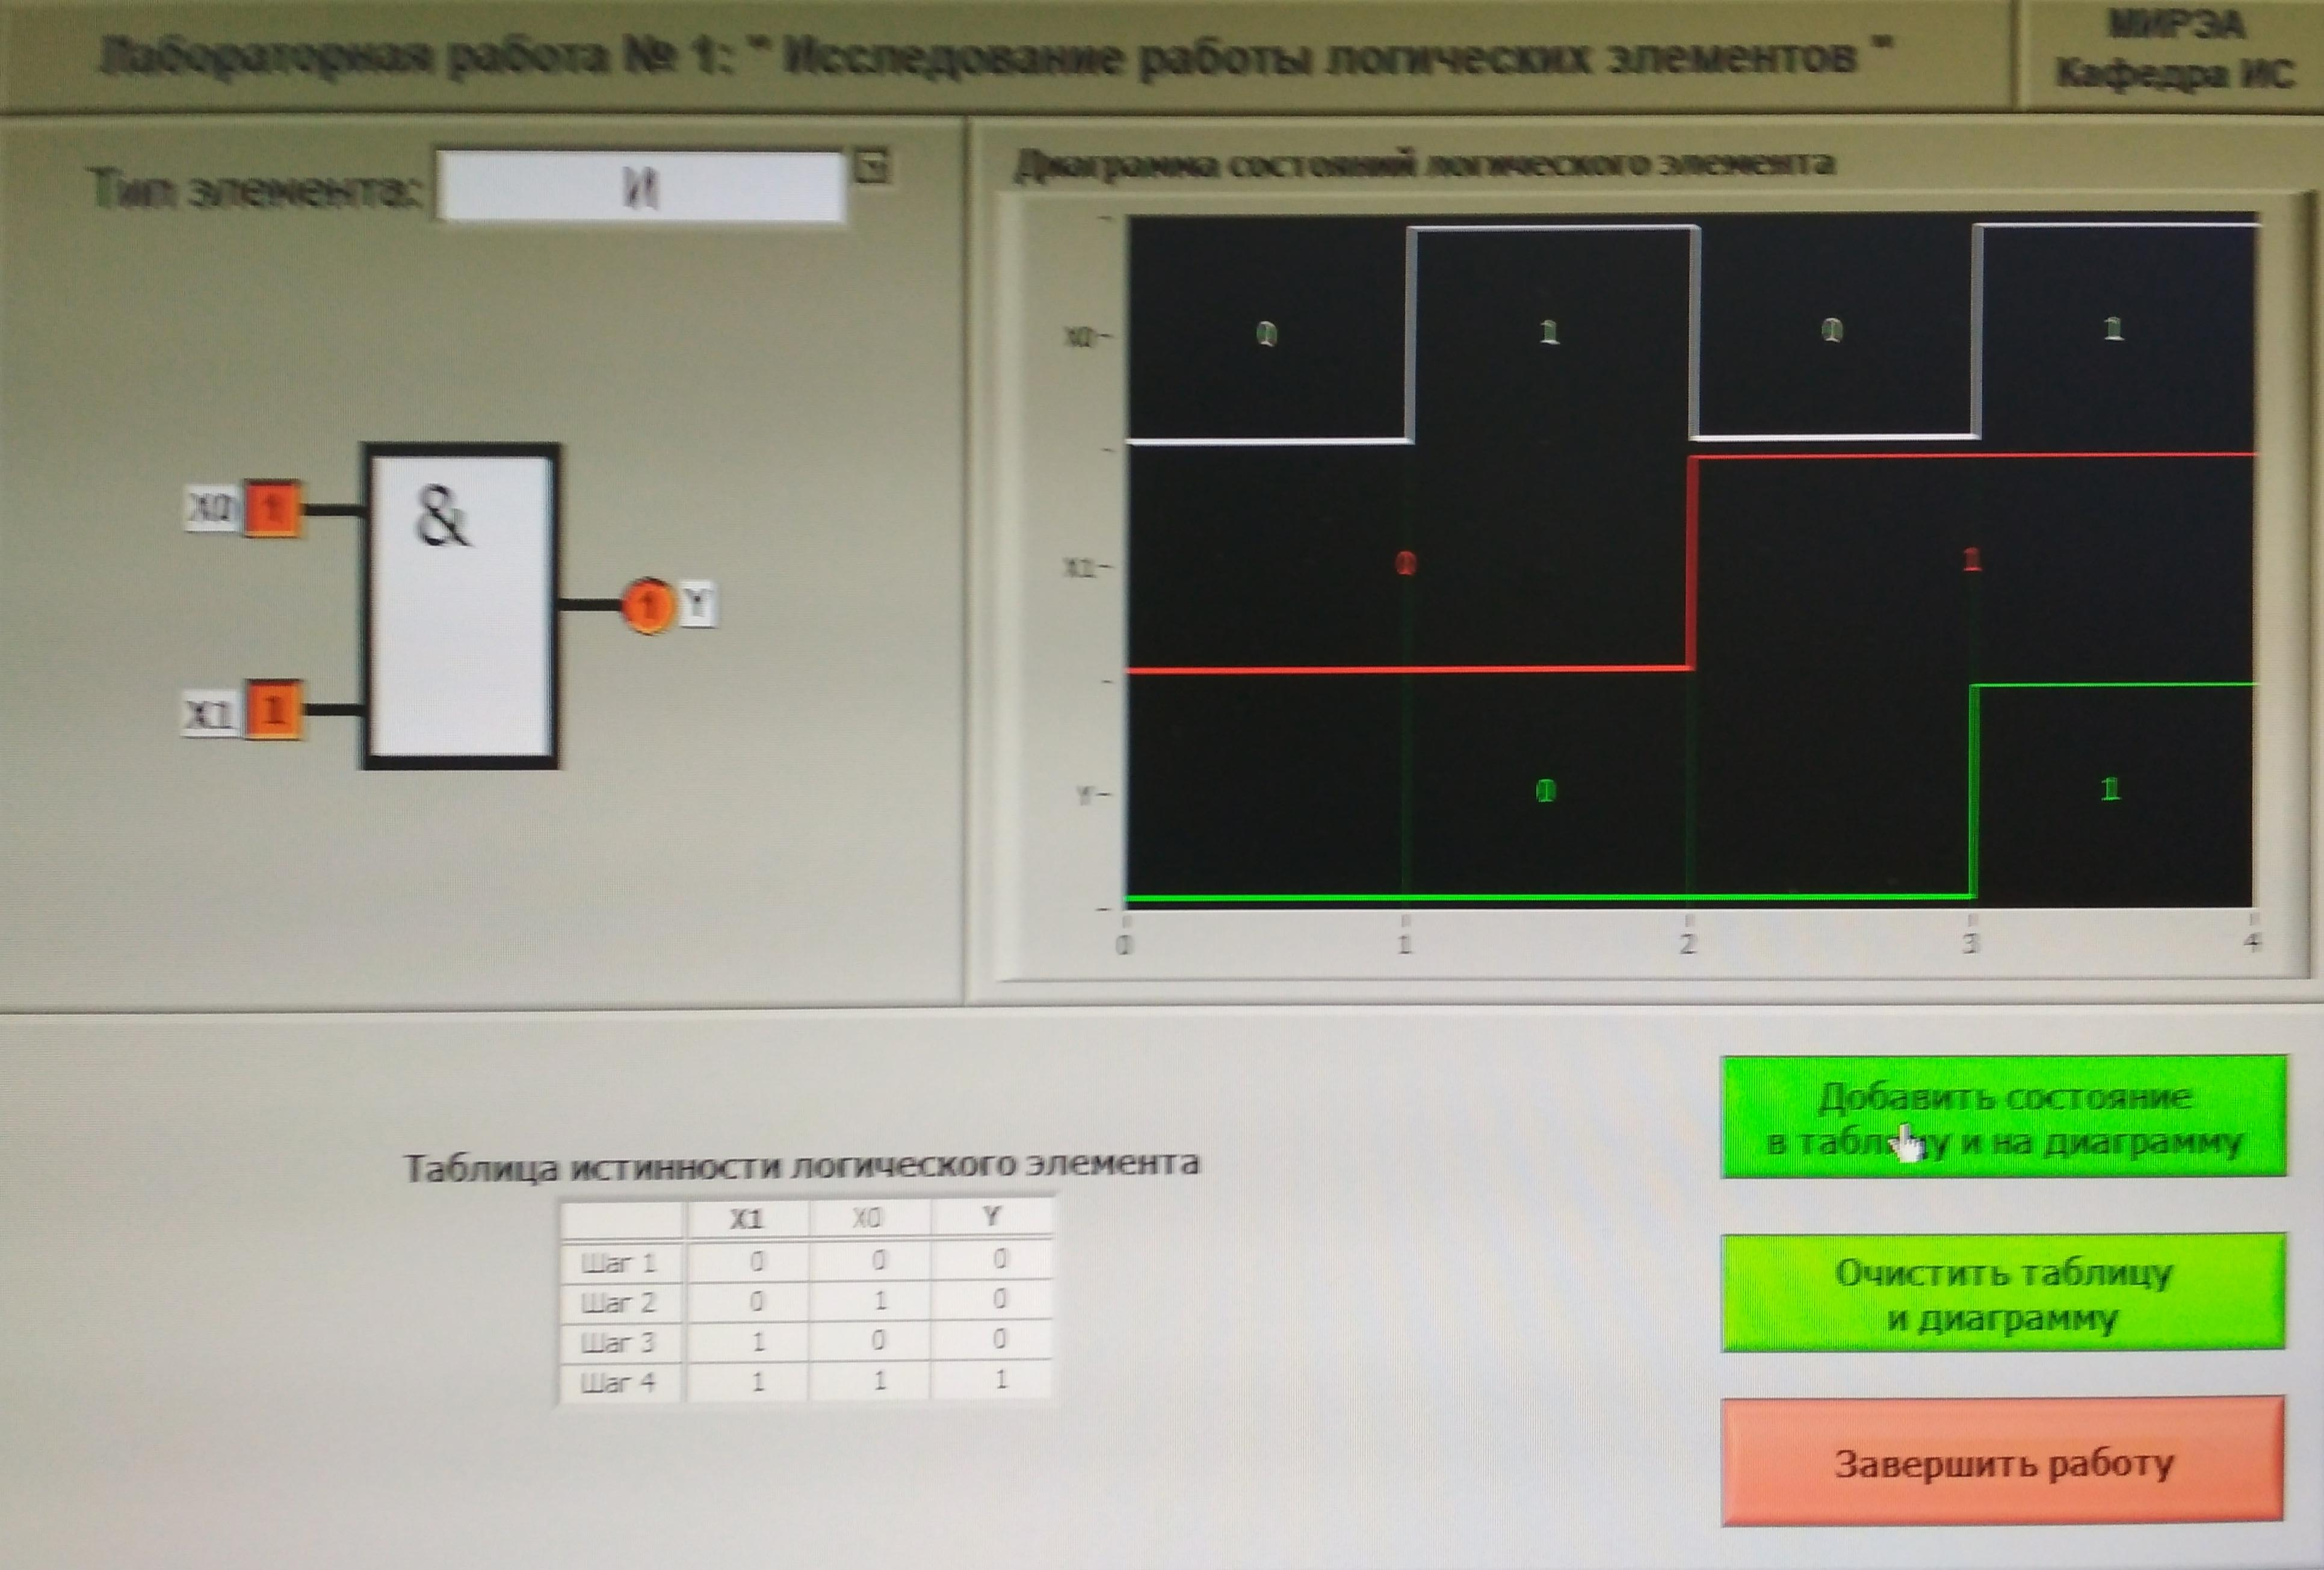
\includegraphics[width=0.85\linewidth]{imgs/1/and}
	\caption{Результат схемы И}
	\label{fig:1_and}
\end{figure}

\begin{figure}[H]
	\centering
	\begin{minipage}{.45\textwidth}
		\centering
		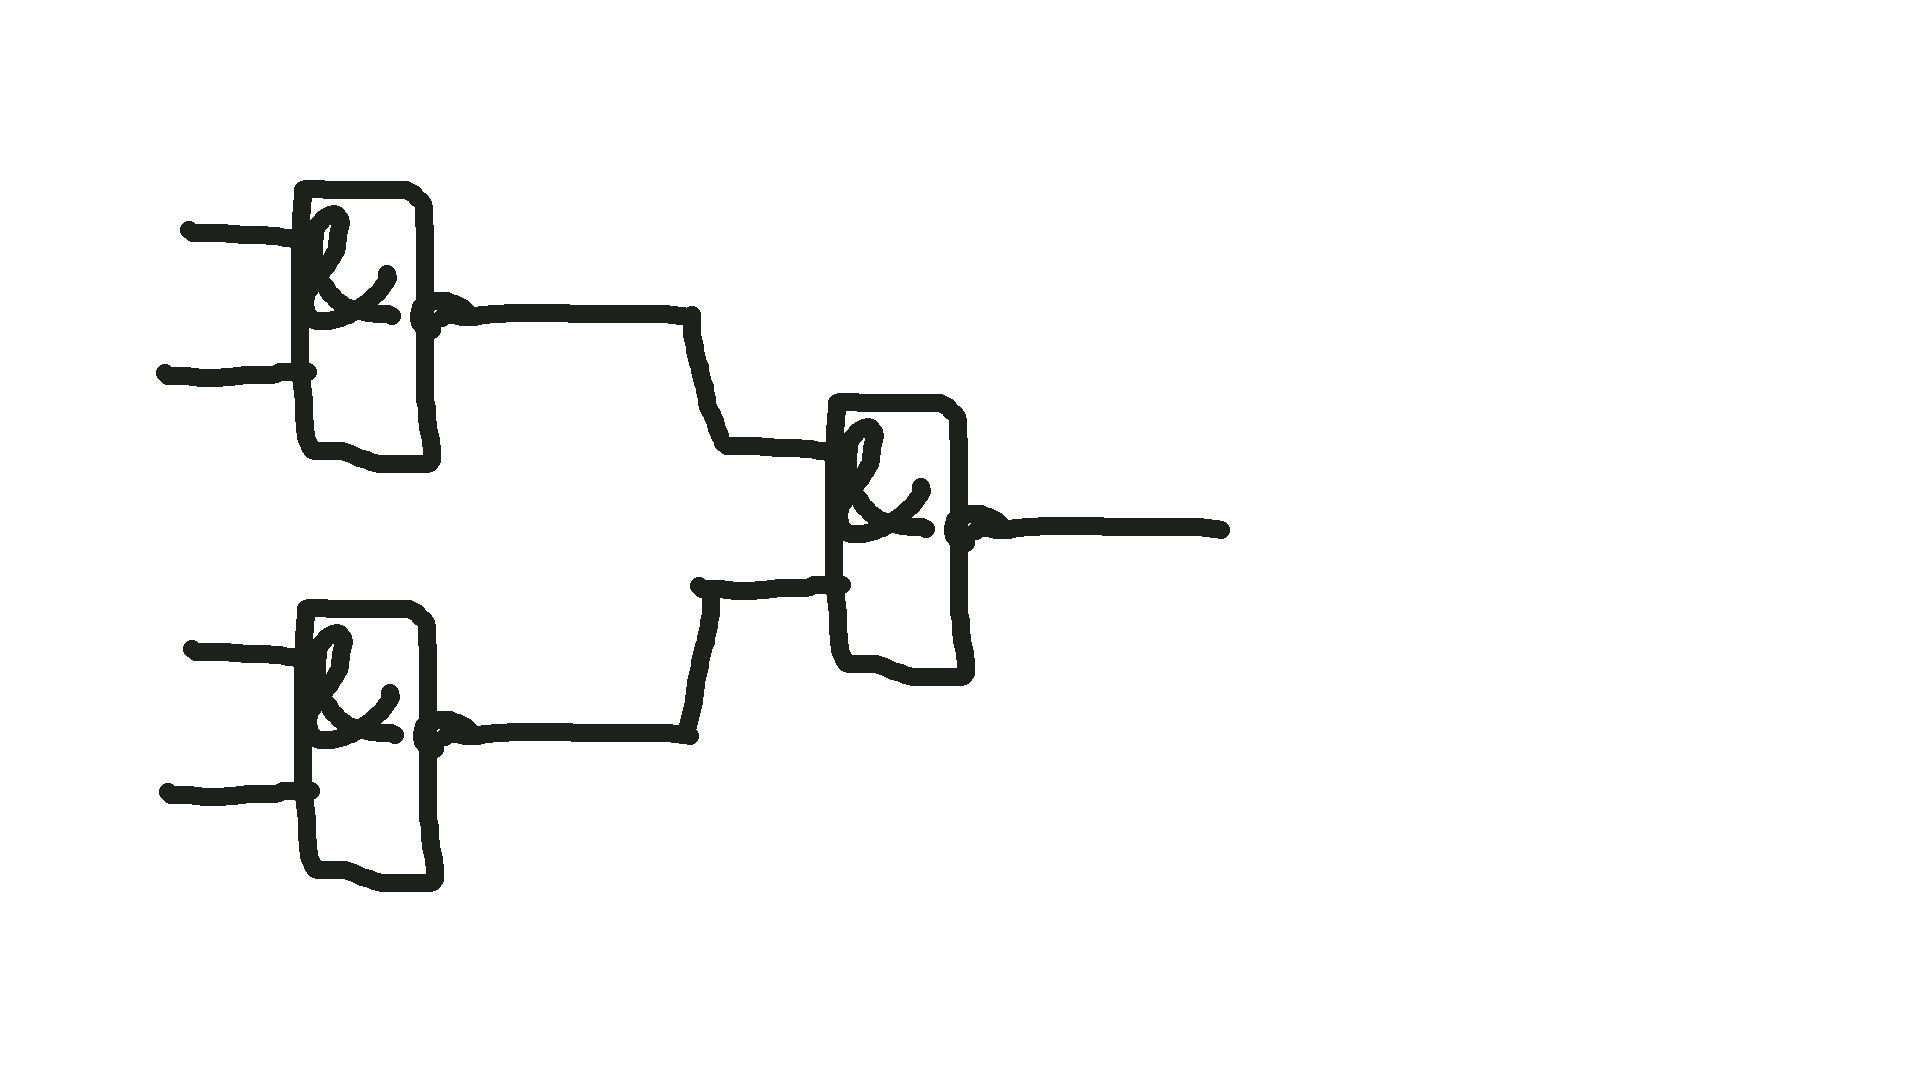
\includegraphics[width=0.85\linewidth]{imgs/1/and_and}
	\end{minipage}
	\begin{minipage}{.45\textwidth}
		\centering
		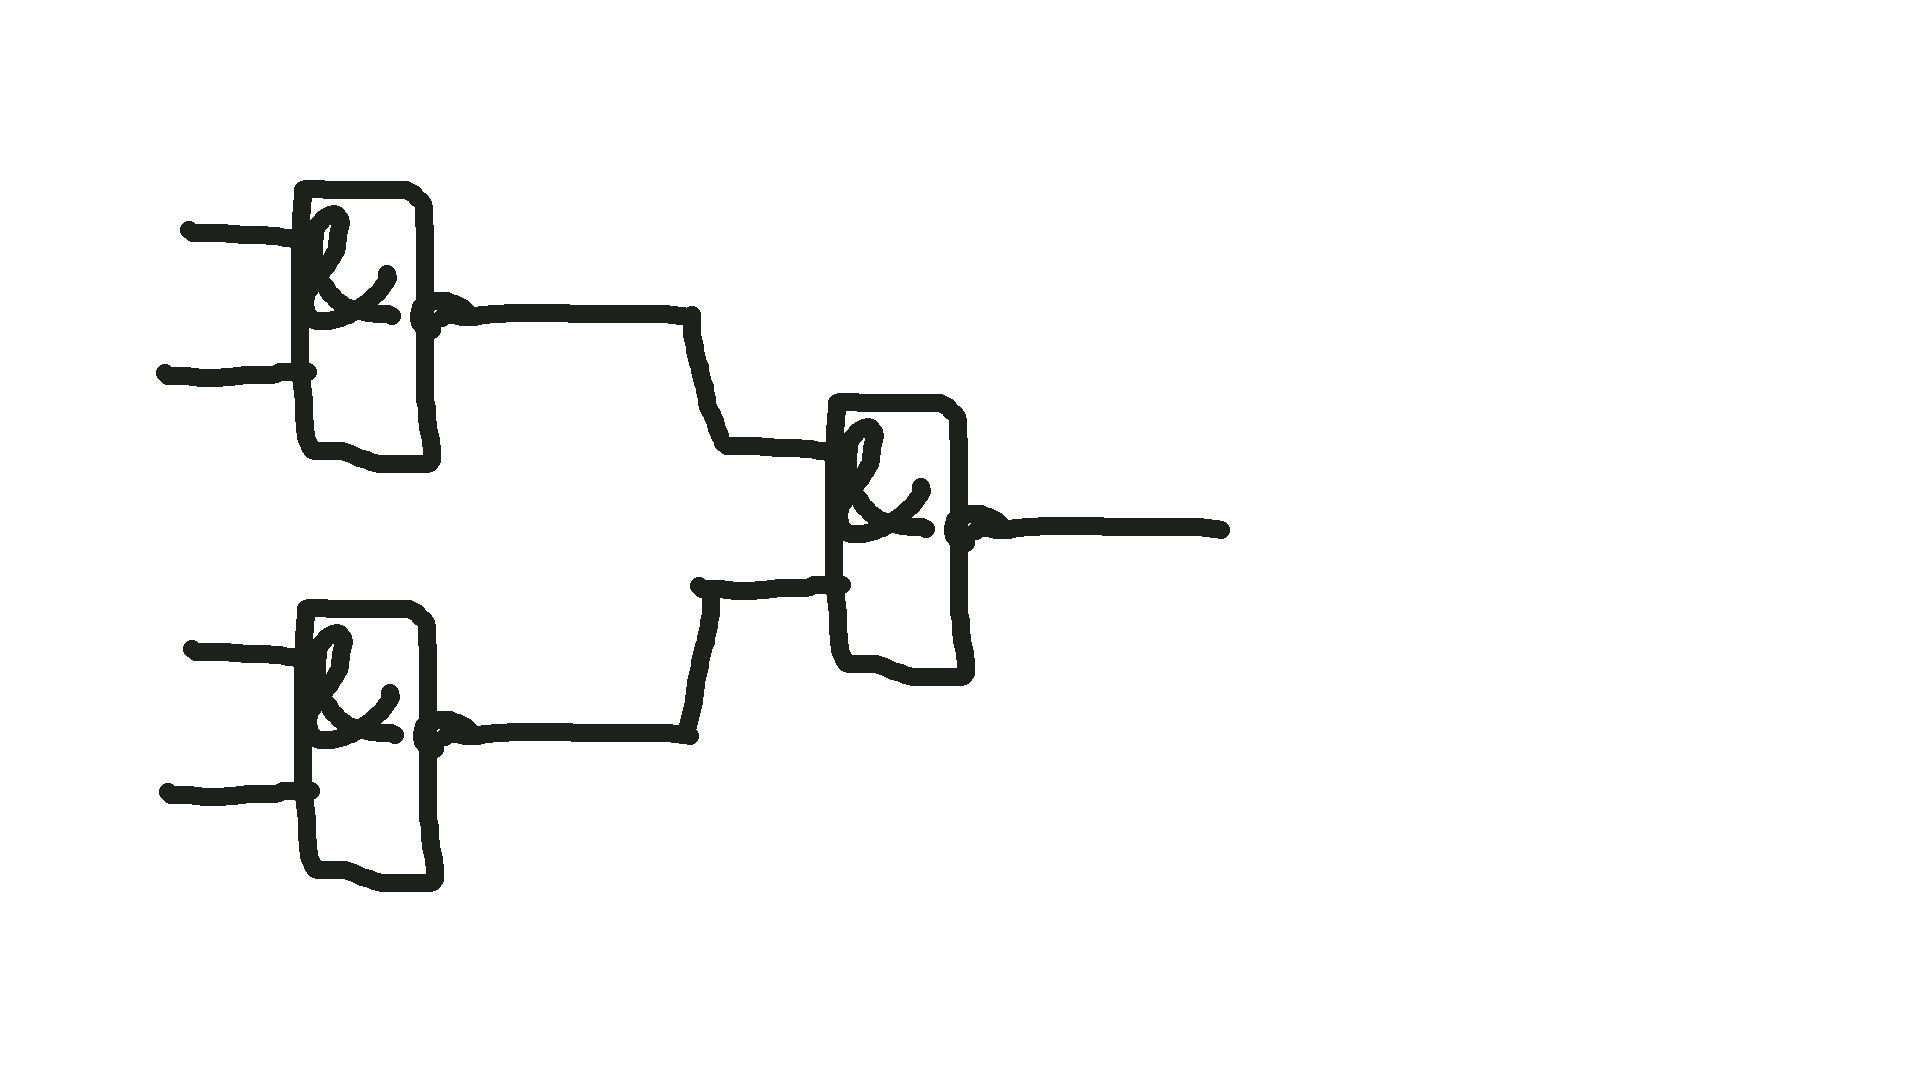
\includegraphics[width=0.85\linewidth]{imgs/1/and_or}
	\end{minipage}
	\caption{Реализация элемента И в базисах 2И-НЕ и 2ИЛИ-НЕ}
\end{figure}


Элемент SN74AHC1G09
 
Характеристики:
\begin{itemize}
	\item Operating Range from 2 V to 5.5 V
	\item Maximum $t_{pd}$ of 6 ns at 5 V
	\item ±8-mA Output Drive at 5 V
\end{itemize}

\subsection{Элемент И-НЕ}

\begin{figure}[H]
	\centering
	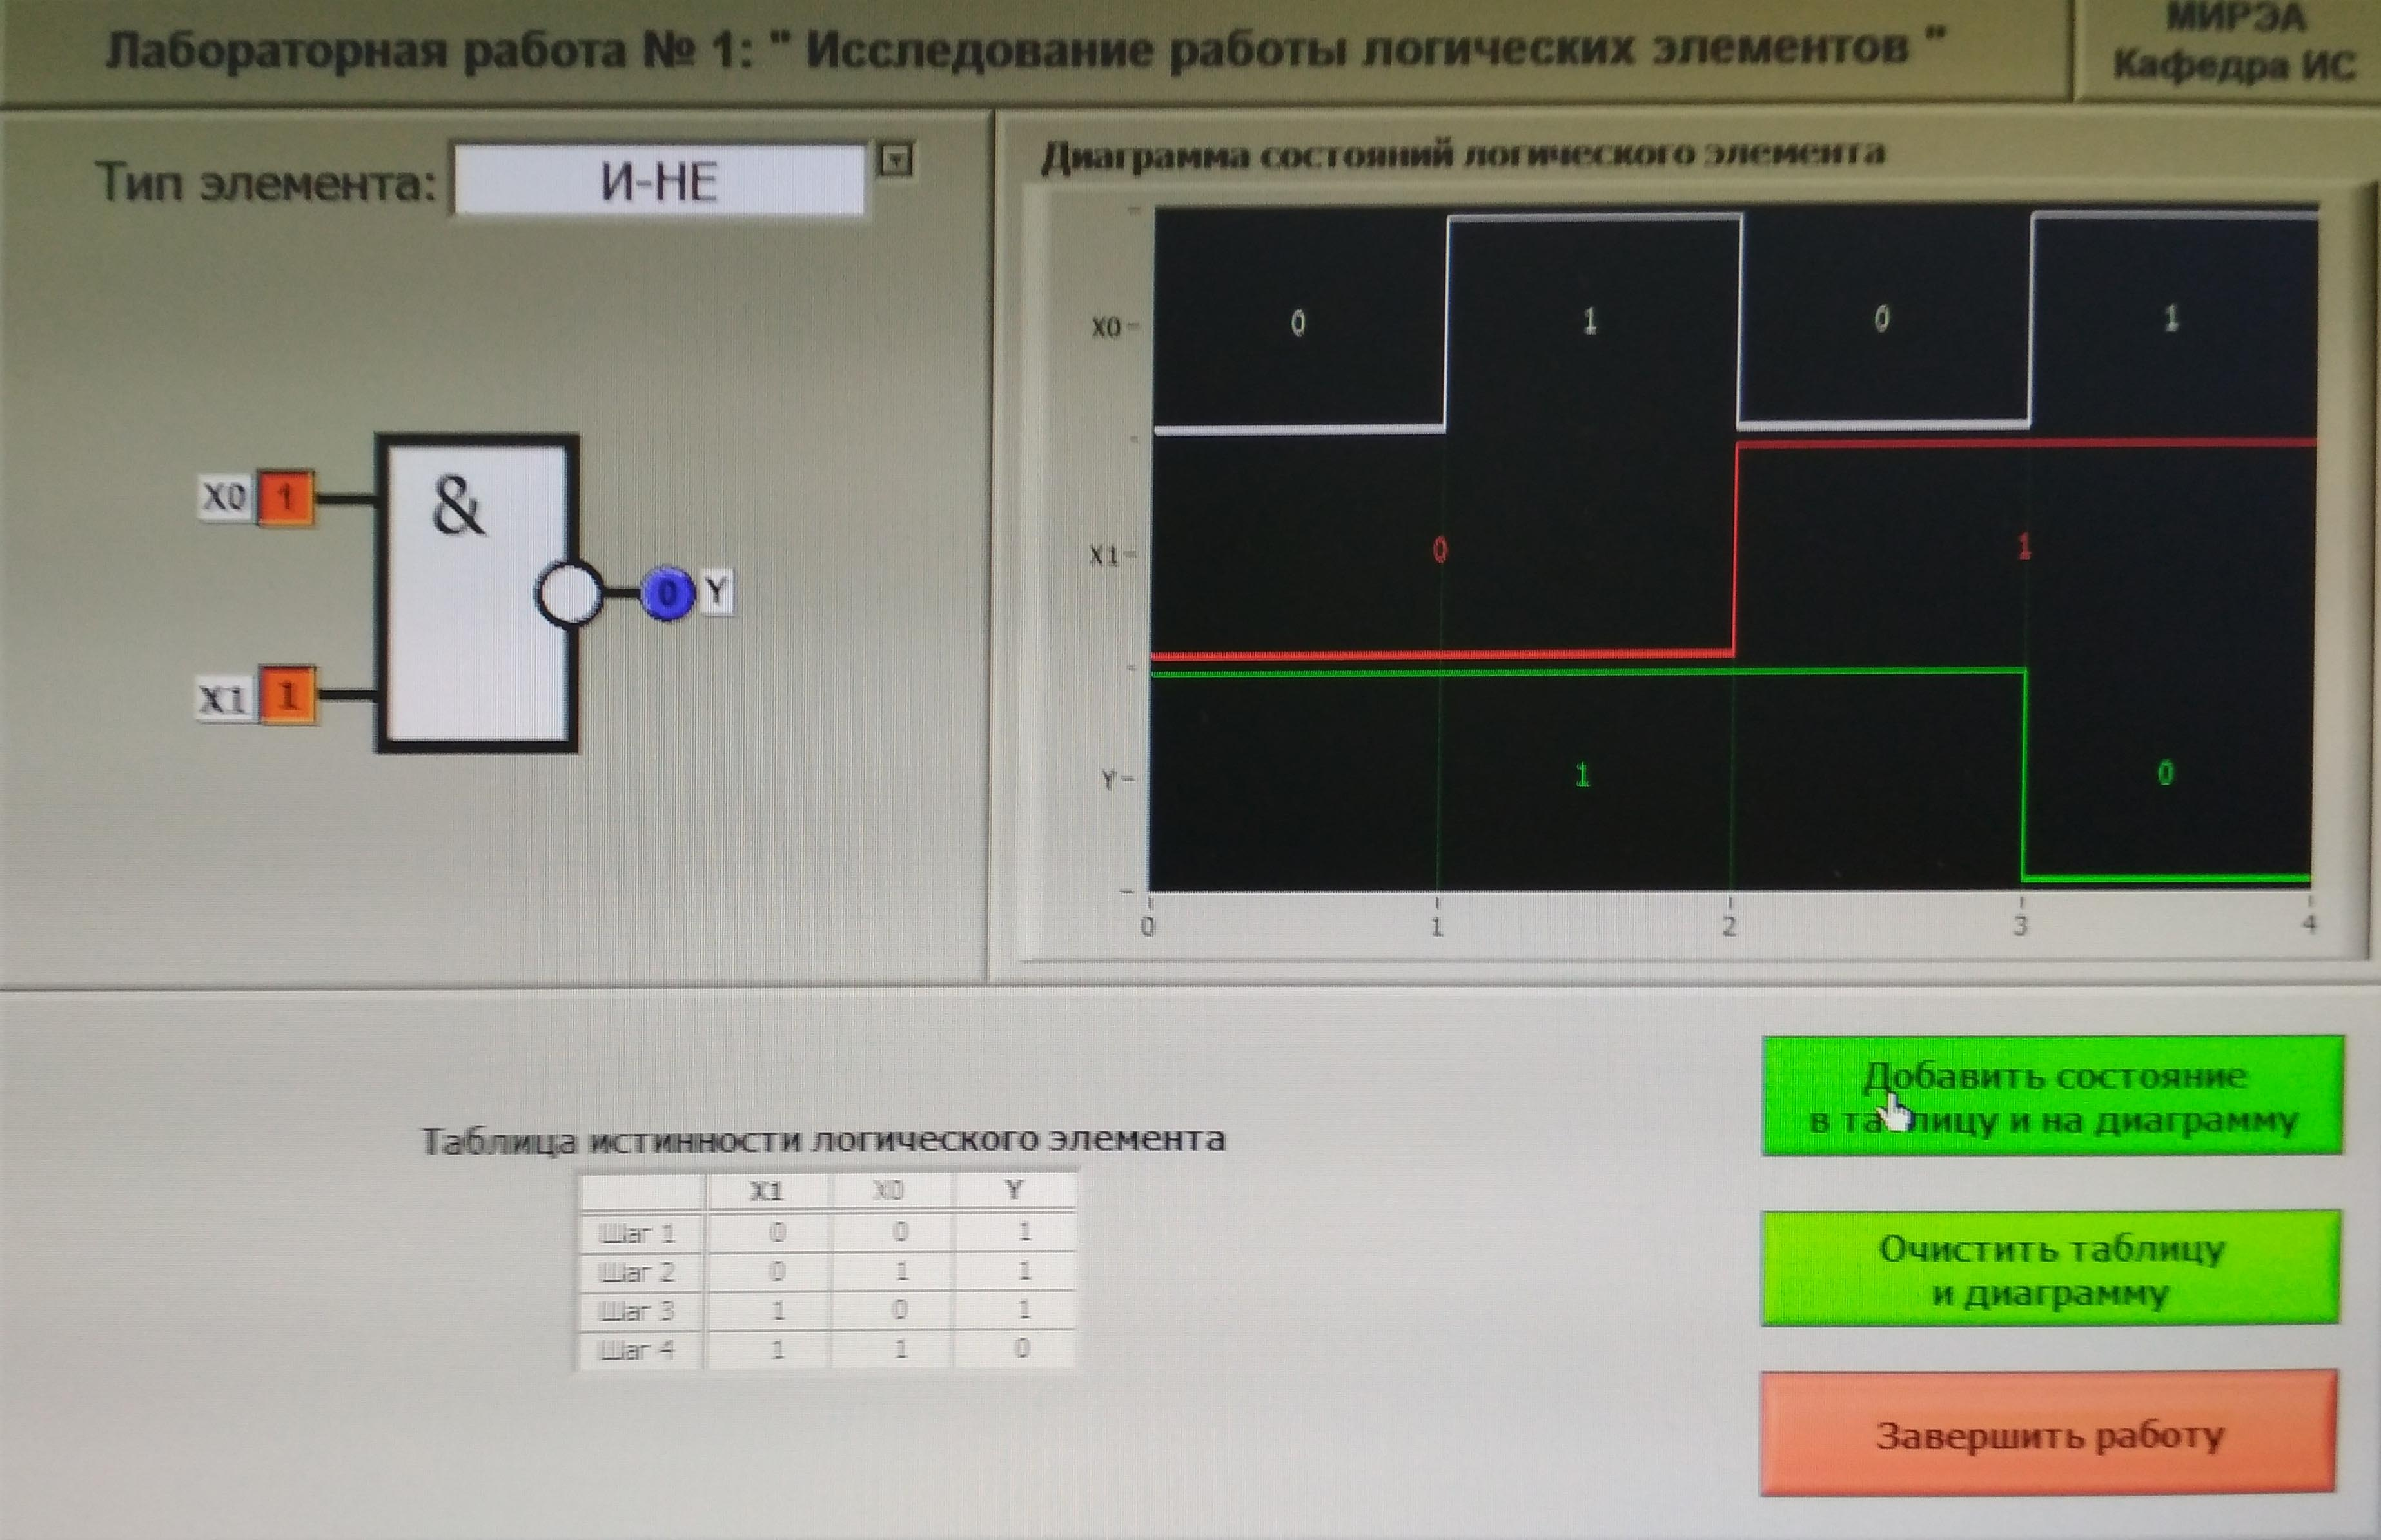
\includegraphics[width=0.85\linewidth]{imgs/1/and-not}
	\caption{Результат схемы И-НЕ}
	\label{fig:1_and-not}
\end{figure}

\begin{figure}[H]
	\centering
	\begin{minipage}{.45\textwidth}
		\centering
		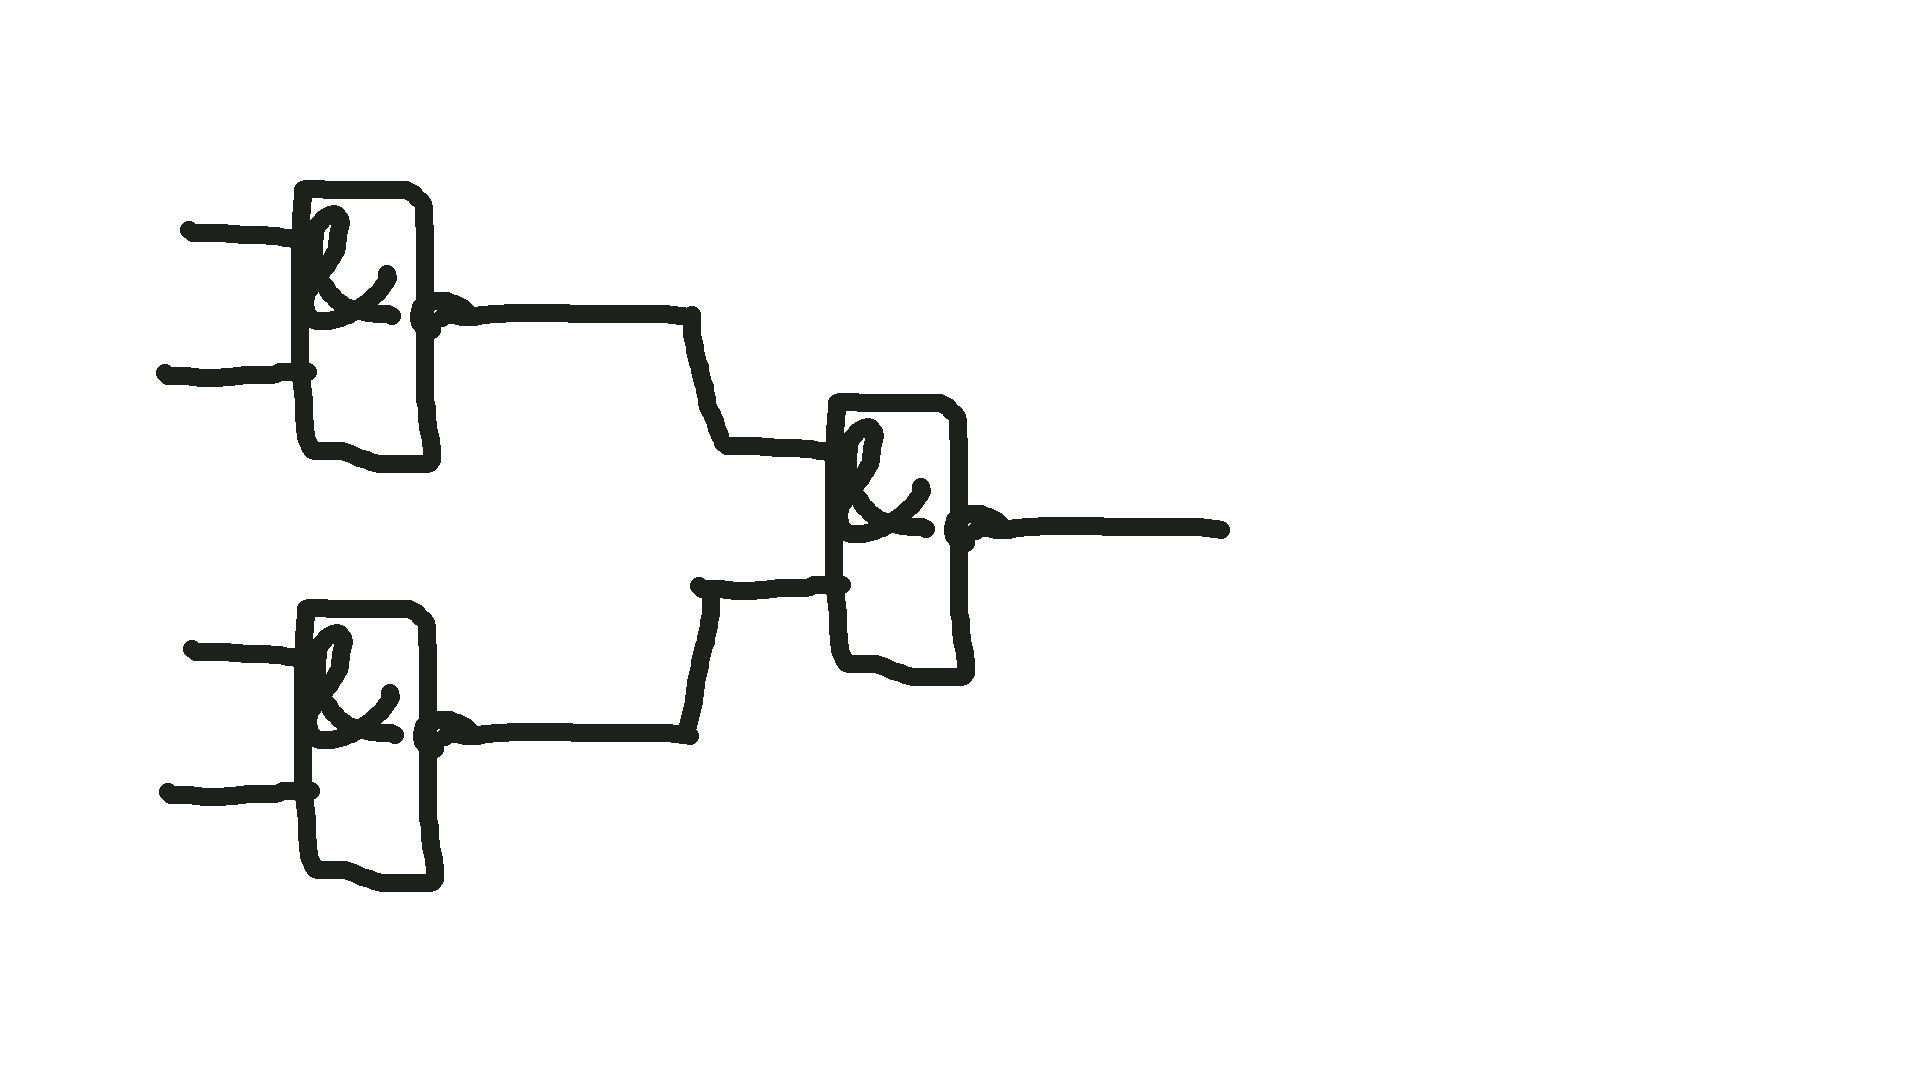
\includegraphics[width=0.85\linewidth]{imgs/1/and-not_and}
	\end{minipage}
	\begin{minipage}{.45\textwidth}
		\centering
		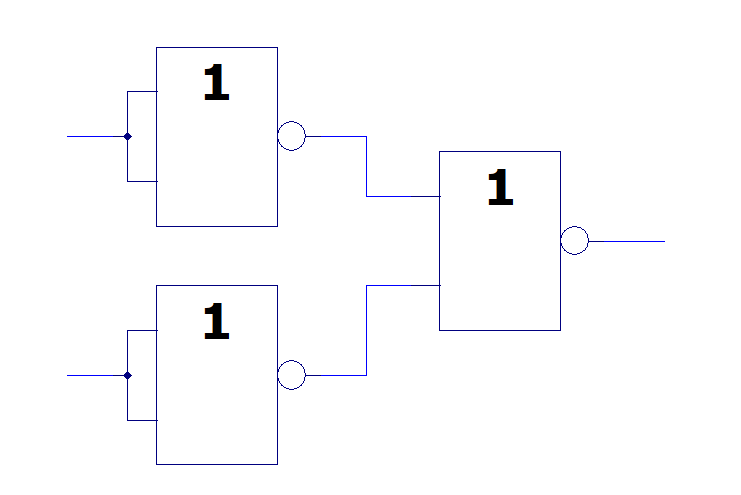
\includegraphics[width=0.85\linewidth]{imgs/1/and-not_or}
	\end{minipage}
	\caption{Реализация элемента И-НЕ в базисах 2И-НЕ и 2ИЛИ-НЕ}
\end{figure}

Элемент SN74AHC1G00-Q1

Характеристики:
\begin{itemize}
	\item Operating Range from 2 V to 5.5 V
	\item Maximum $t_{pd}$ of 6.5 ns at 5 V
	\item ±8-mA Output Drive at 5 V
\end{itemize}

\subsection{Элемент ИЛИ}

\begin{figure}[H]
	\centering
	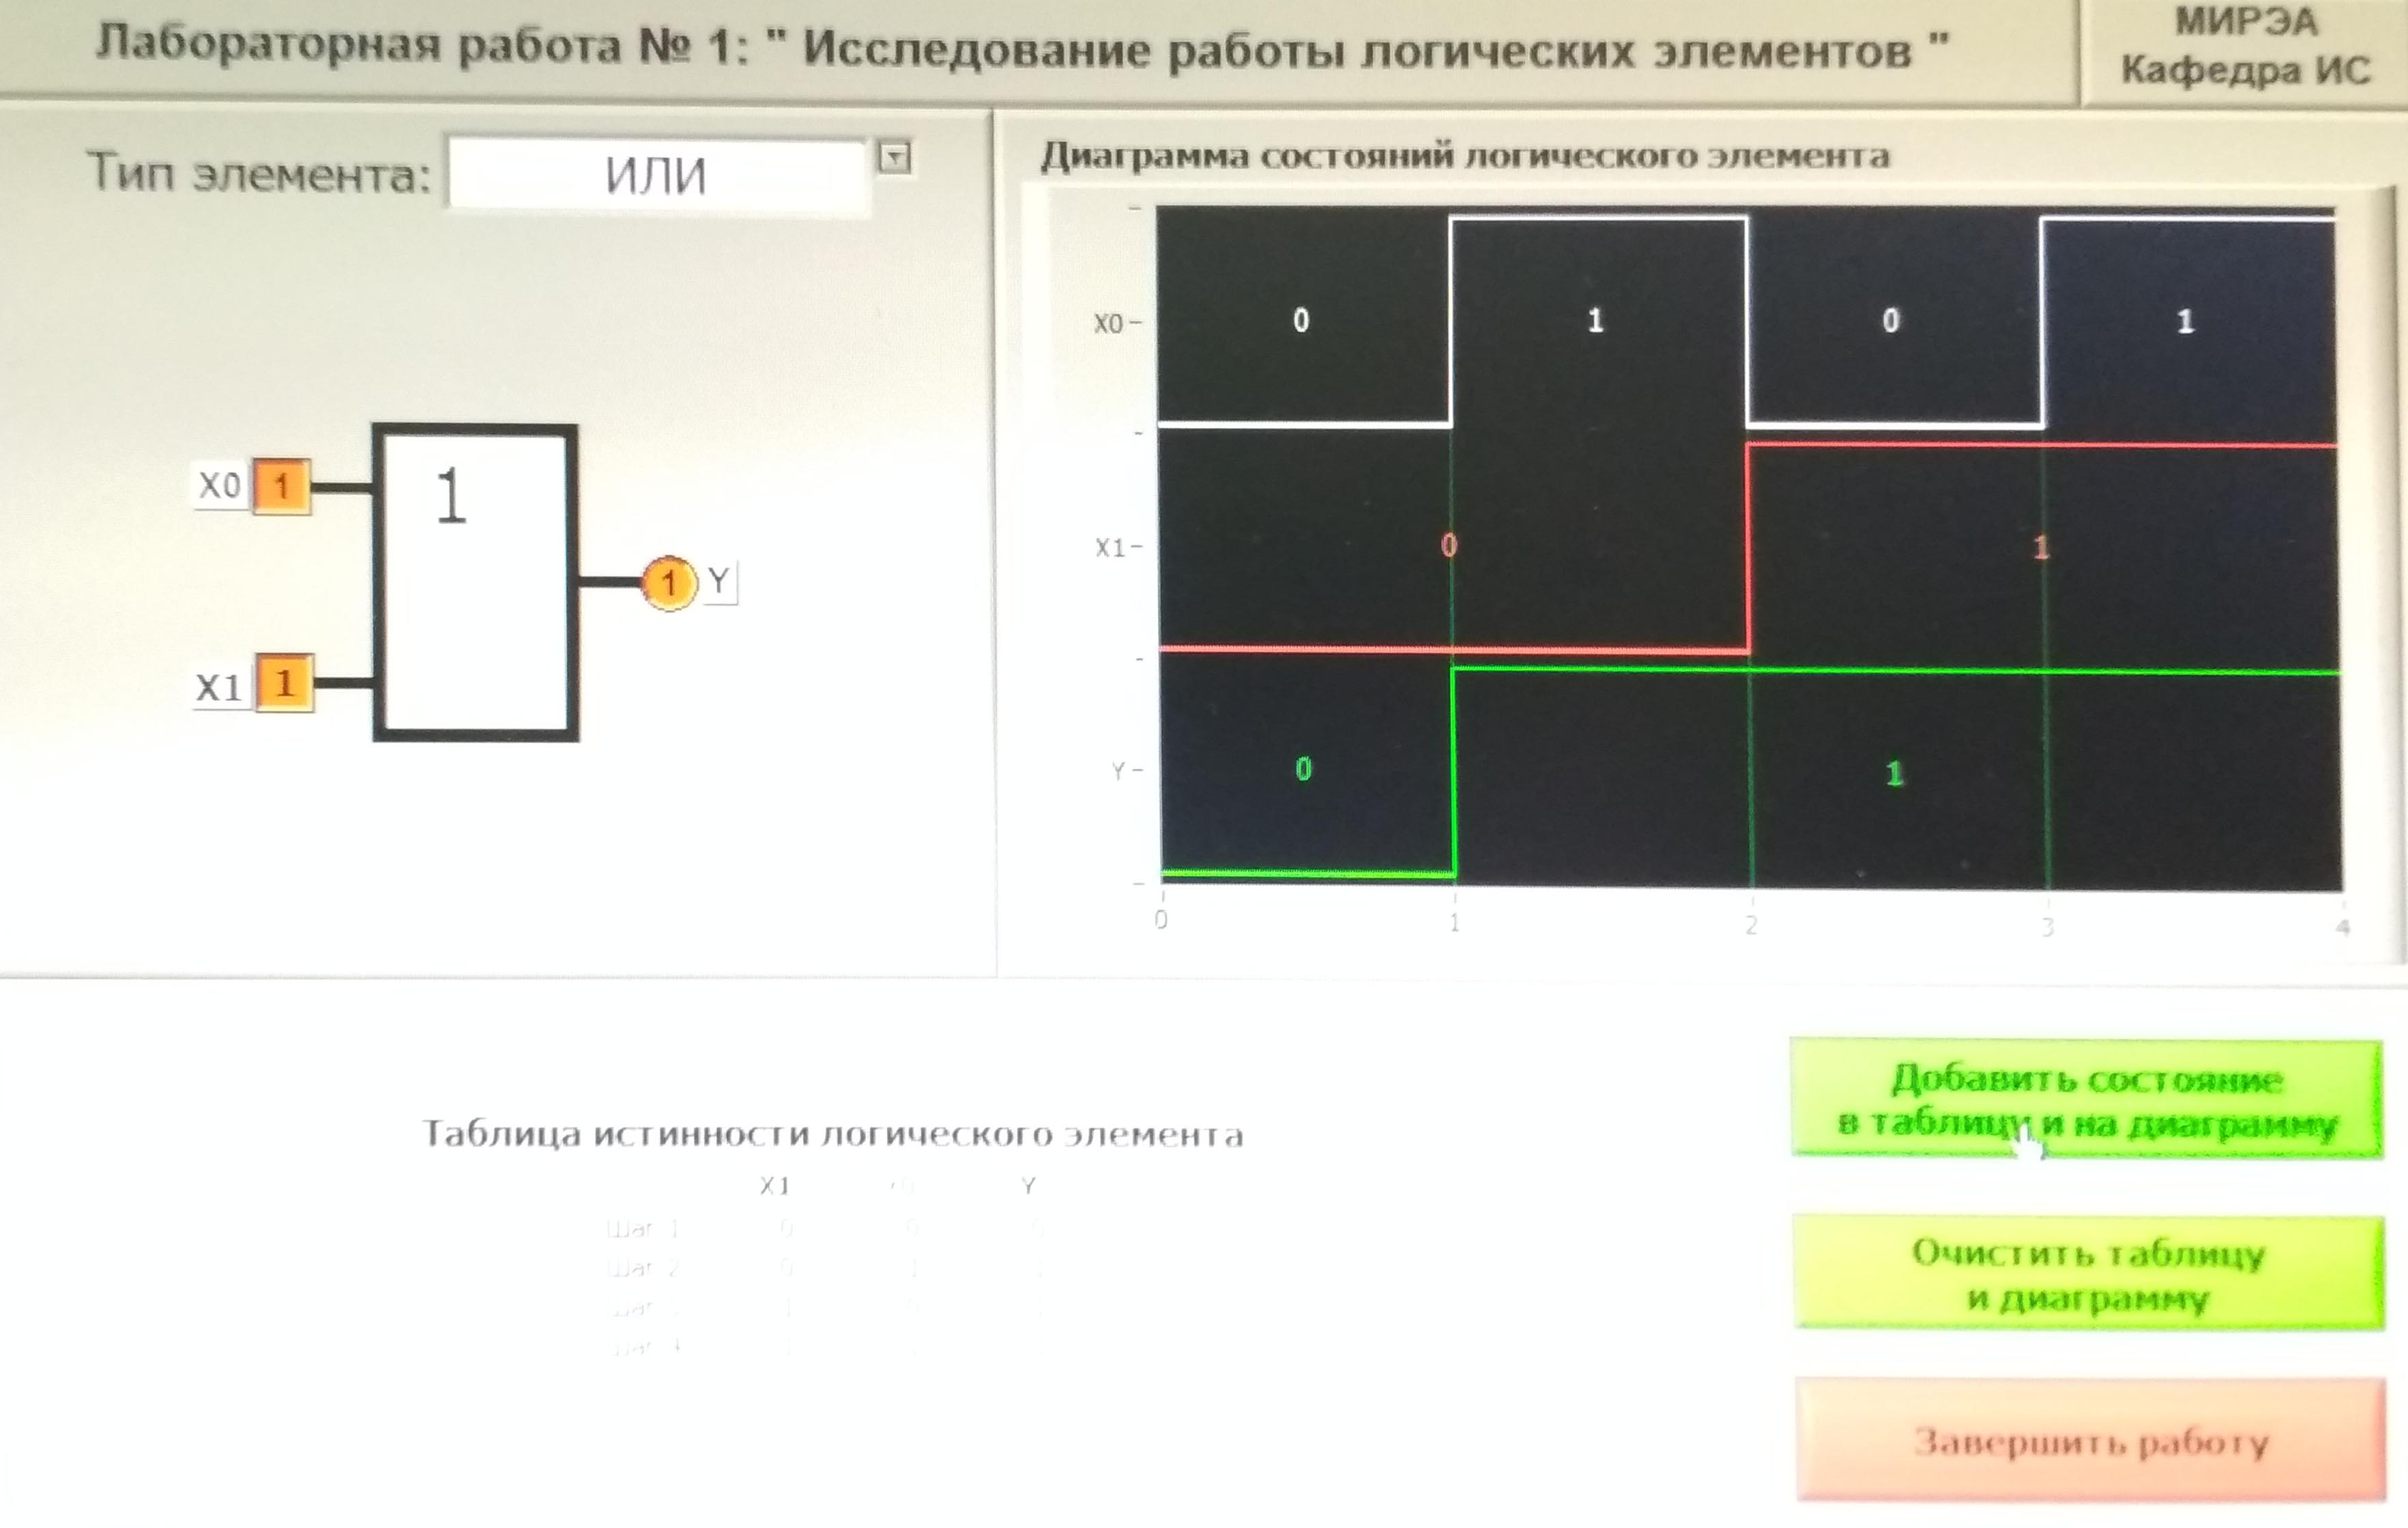
\includegraphics[width=0.85\linewidth]{imgs/1/or}
	\caption{Результат схемы ИЛИ}
	\label{fig:1_or}
\end{figure}

\begin{figure}[H]
	\centering
	\begin{minipage}{.45\textwidth}
		\centering
		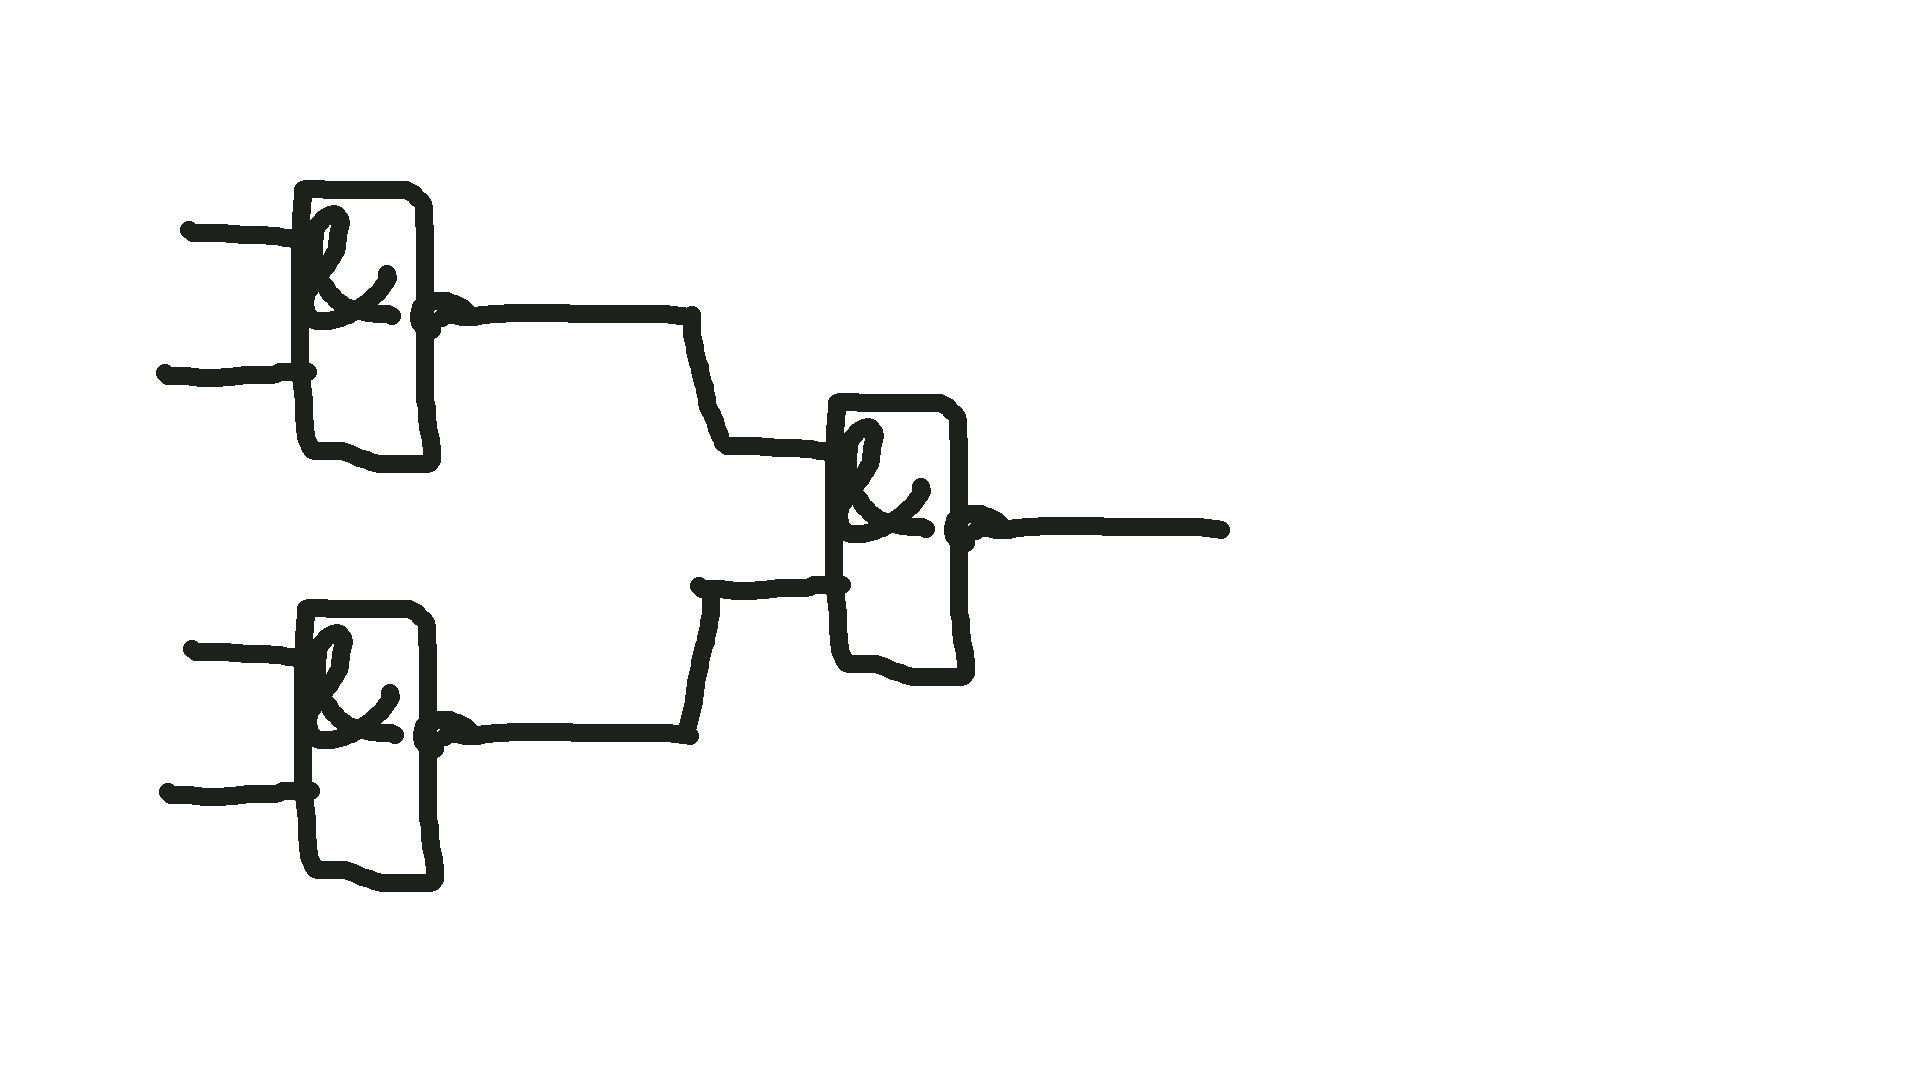
\includegraphics[width=0.85\linewidth]{imgs/1/or_and}
	\end{minipage}
	\begin{minipage}{.45\textwidth}
		\centering
		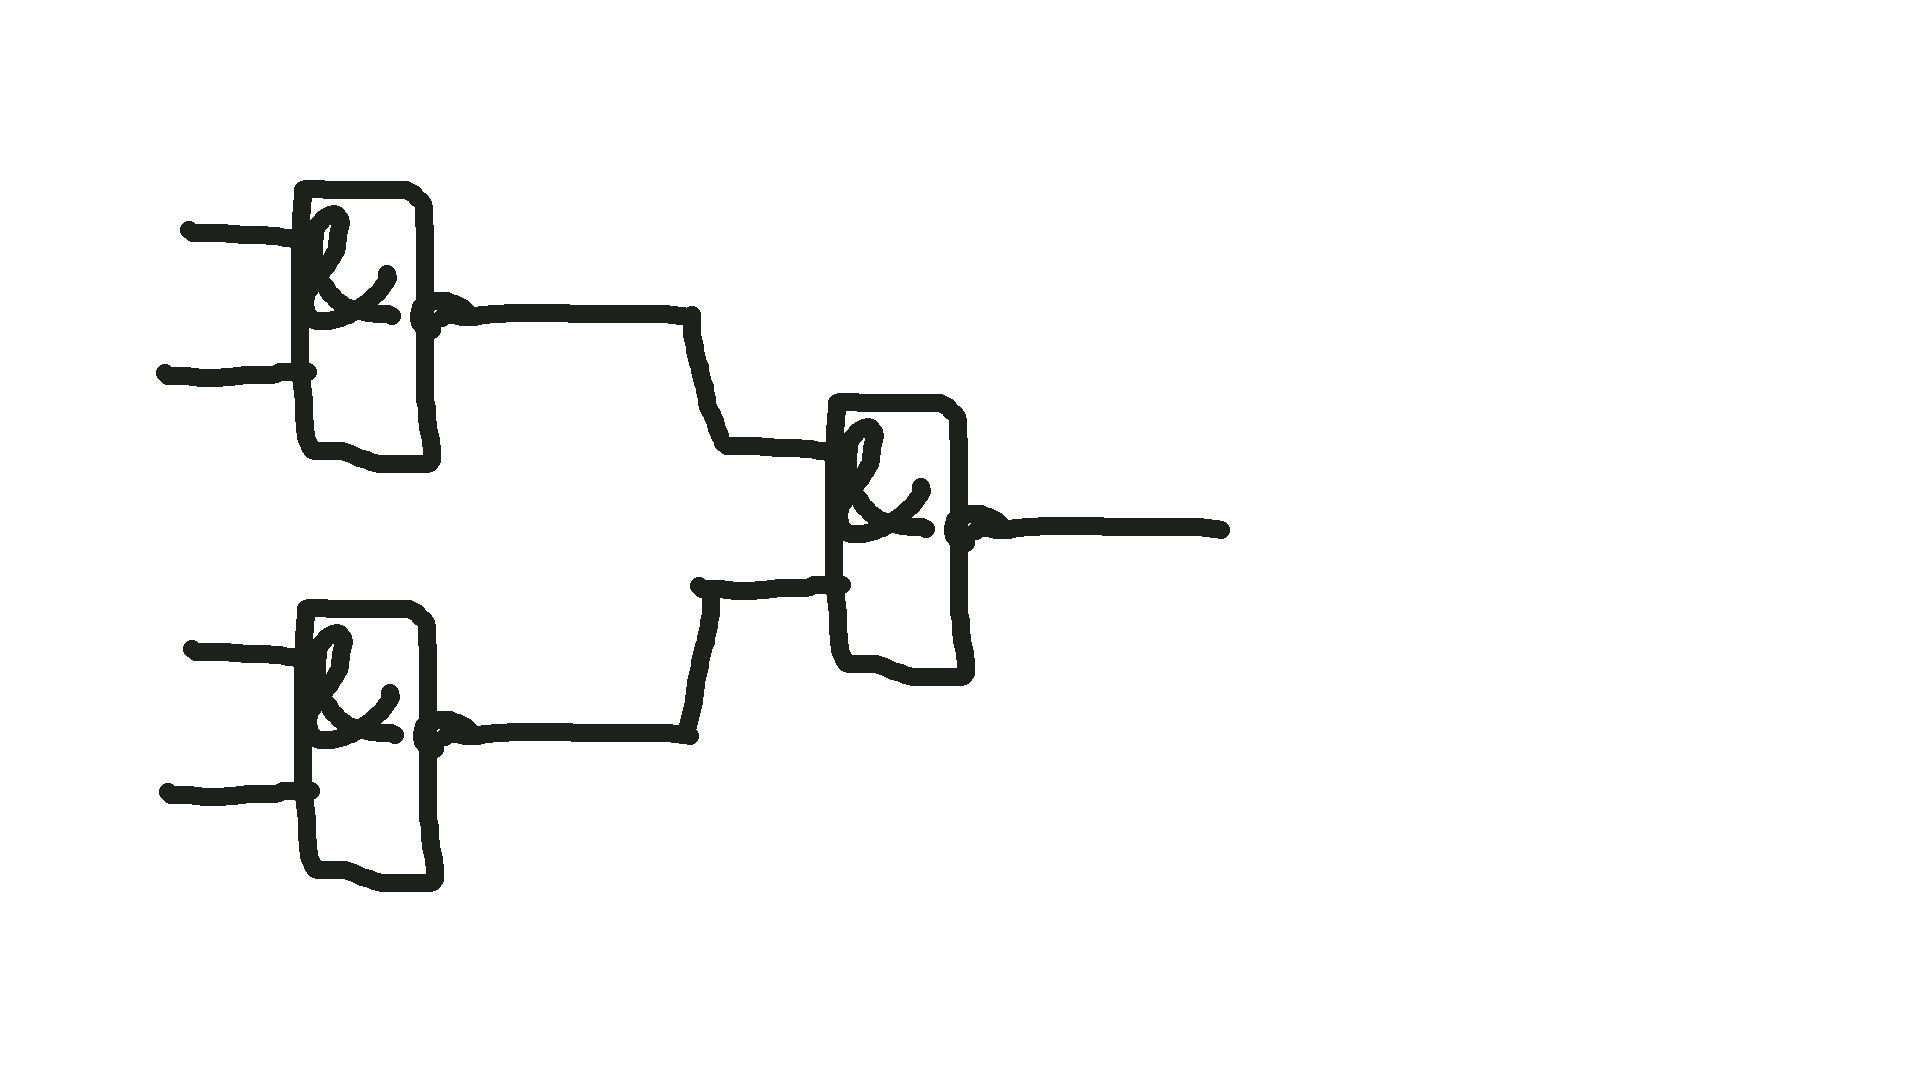
\includegraphics[width=0.85\linewidth]{imgs/1/or_or}
	\end{minipage}
	\caption{Реализация элемента ИЛИ в базисах 2И-НЕ и 2ИЛИ-НЕ}
\end{figure}

Элемент SN74AHCT1G32-Q1

Характеристики:
\begin{itemize}
	\item Operating Range from 4.5 V to 5.5 V
	\item Maximum $t_{pd}$ of 9.5 ns at 5 V
	\item ±8-mA Output Drive at 5 V
\end{itemize}

\subsection{Элемент ИЛИ-НЕ}

\begin{figure}[H]
	\centering
	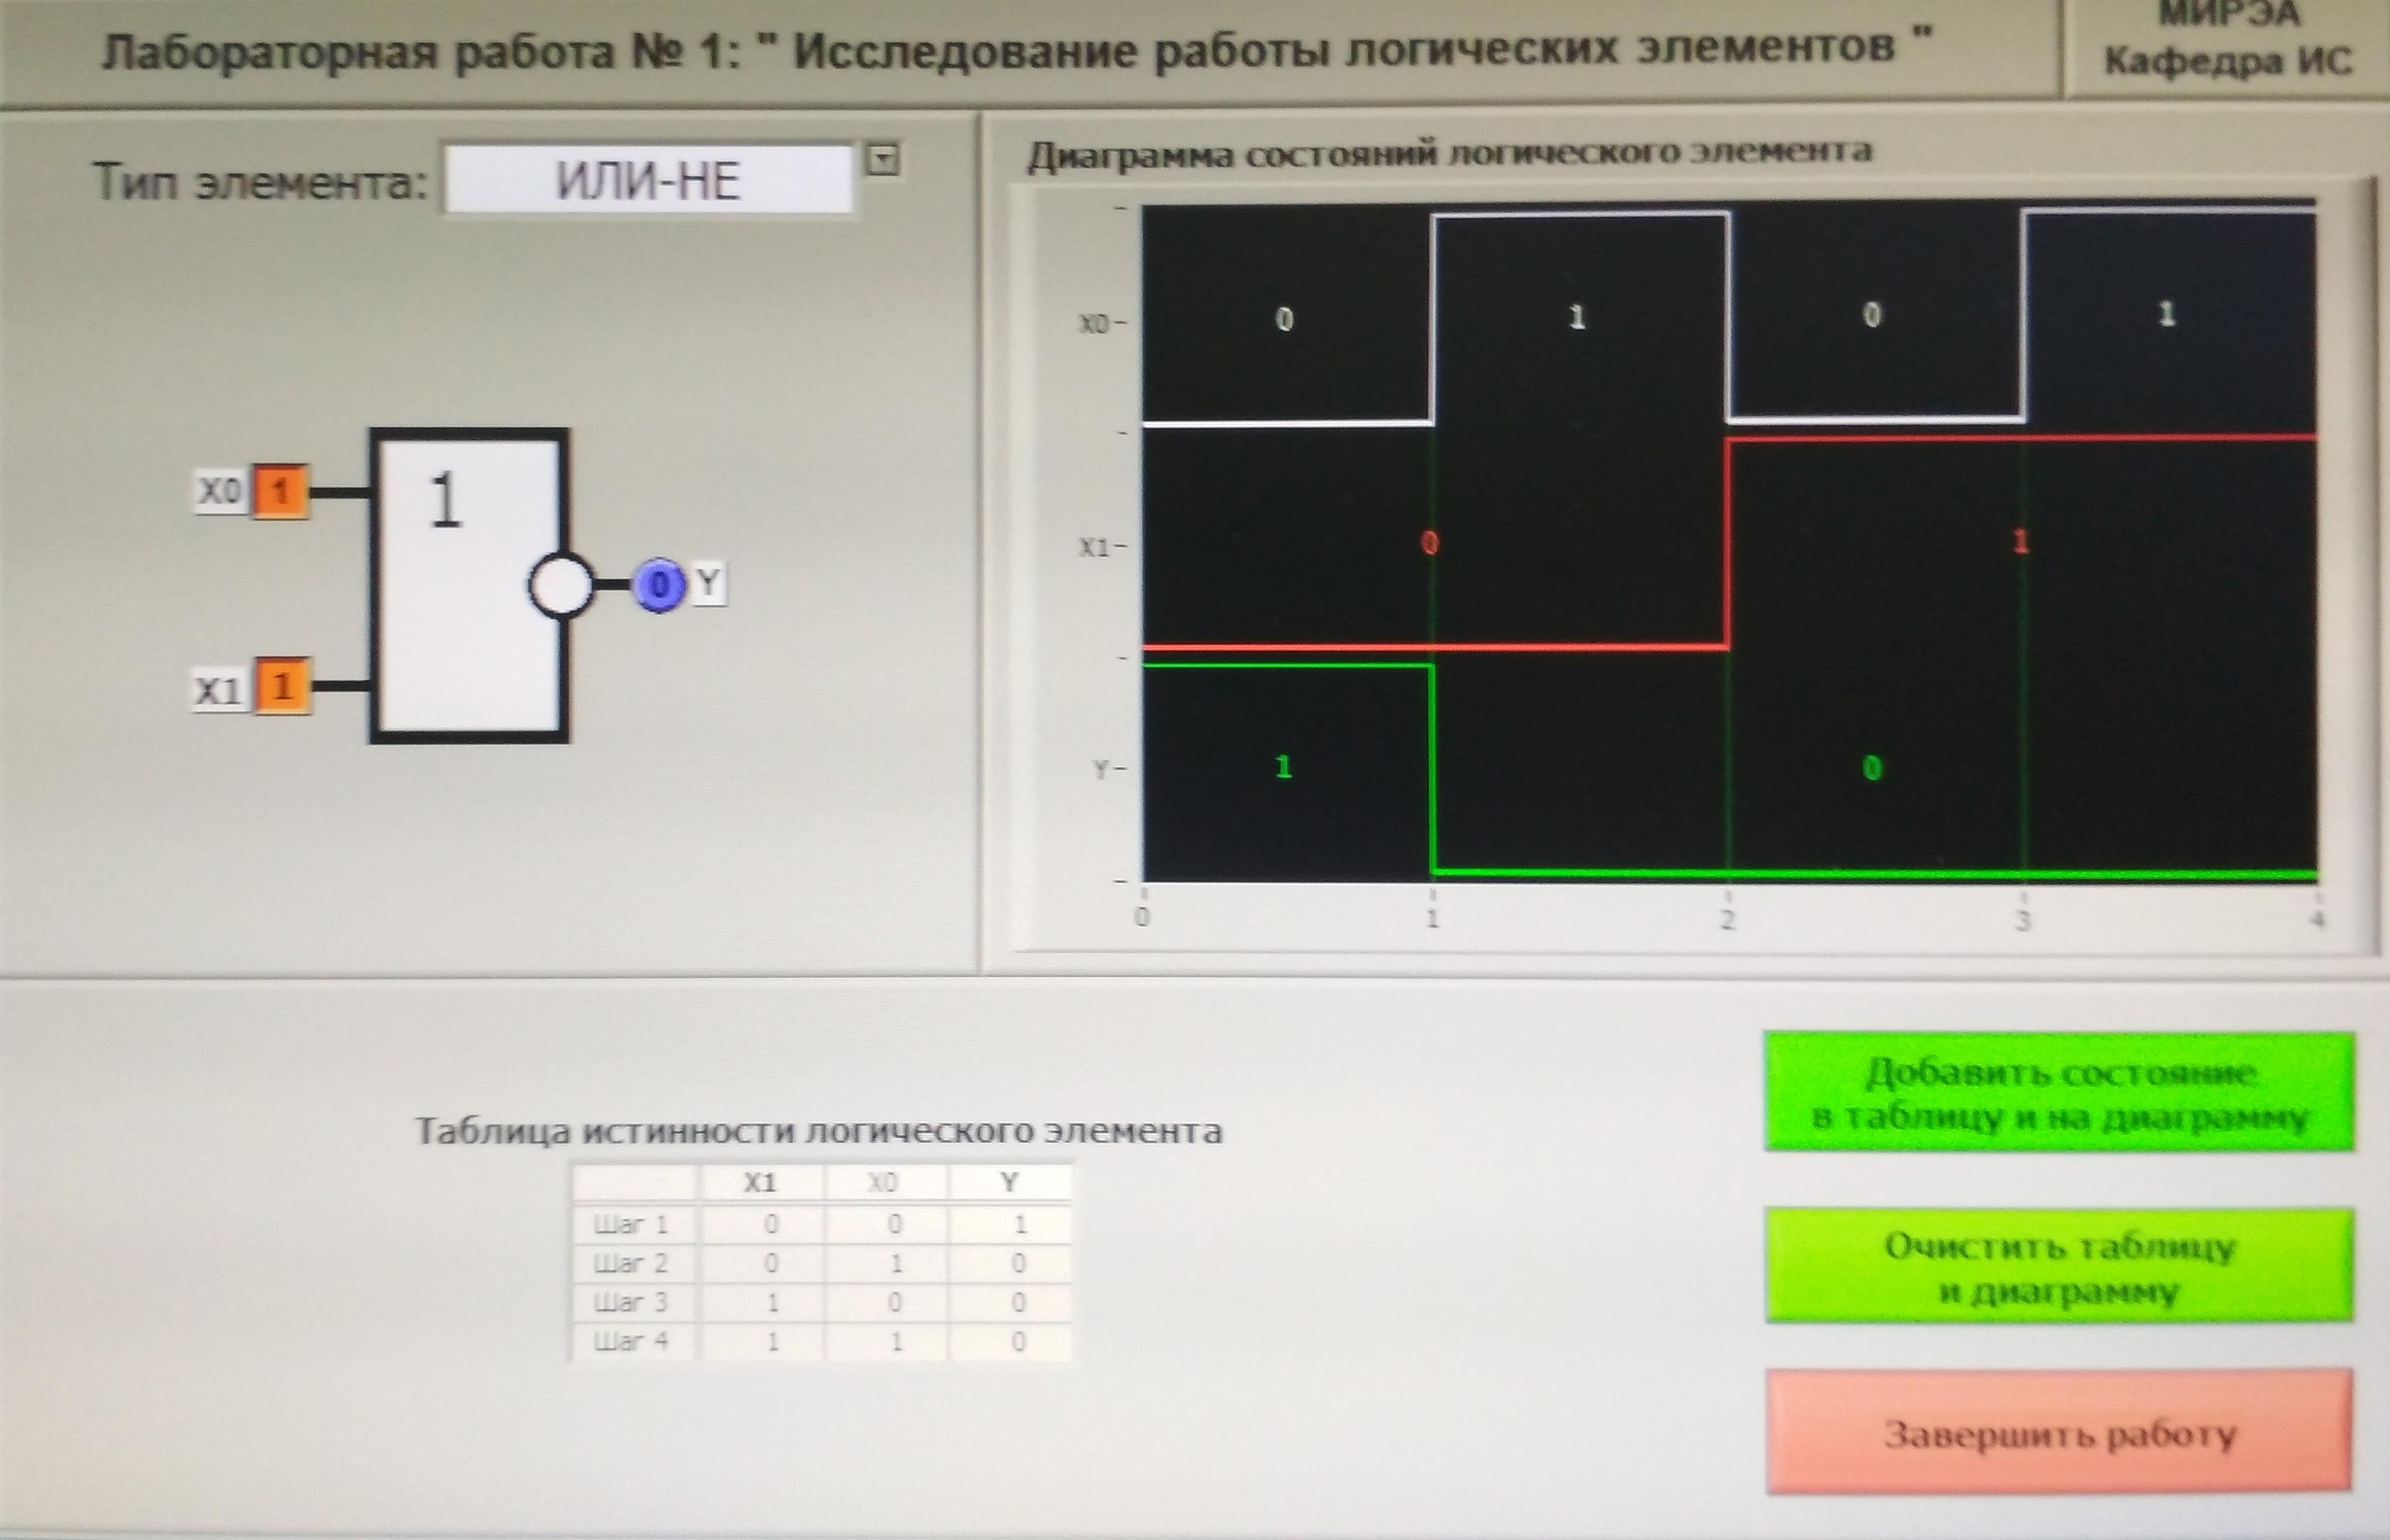
\includegraphics[width=0.85\linewidth]{imgs/1/or-not}
	\caption{Результат схемы ИЛИ-НЕ}
	\label{fig:1_or-not}
\end{figure}

\begin{figure}[H]
	\centering
	\begin{minipage}{.45\textwidth}
		\centering
		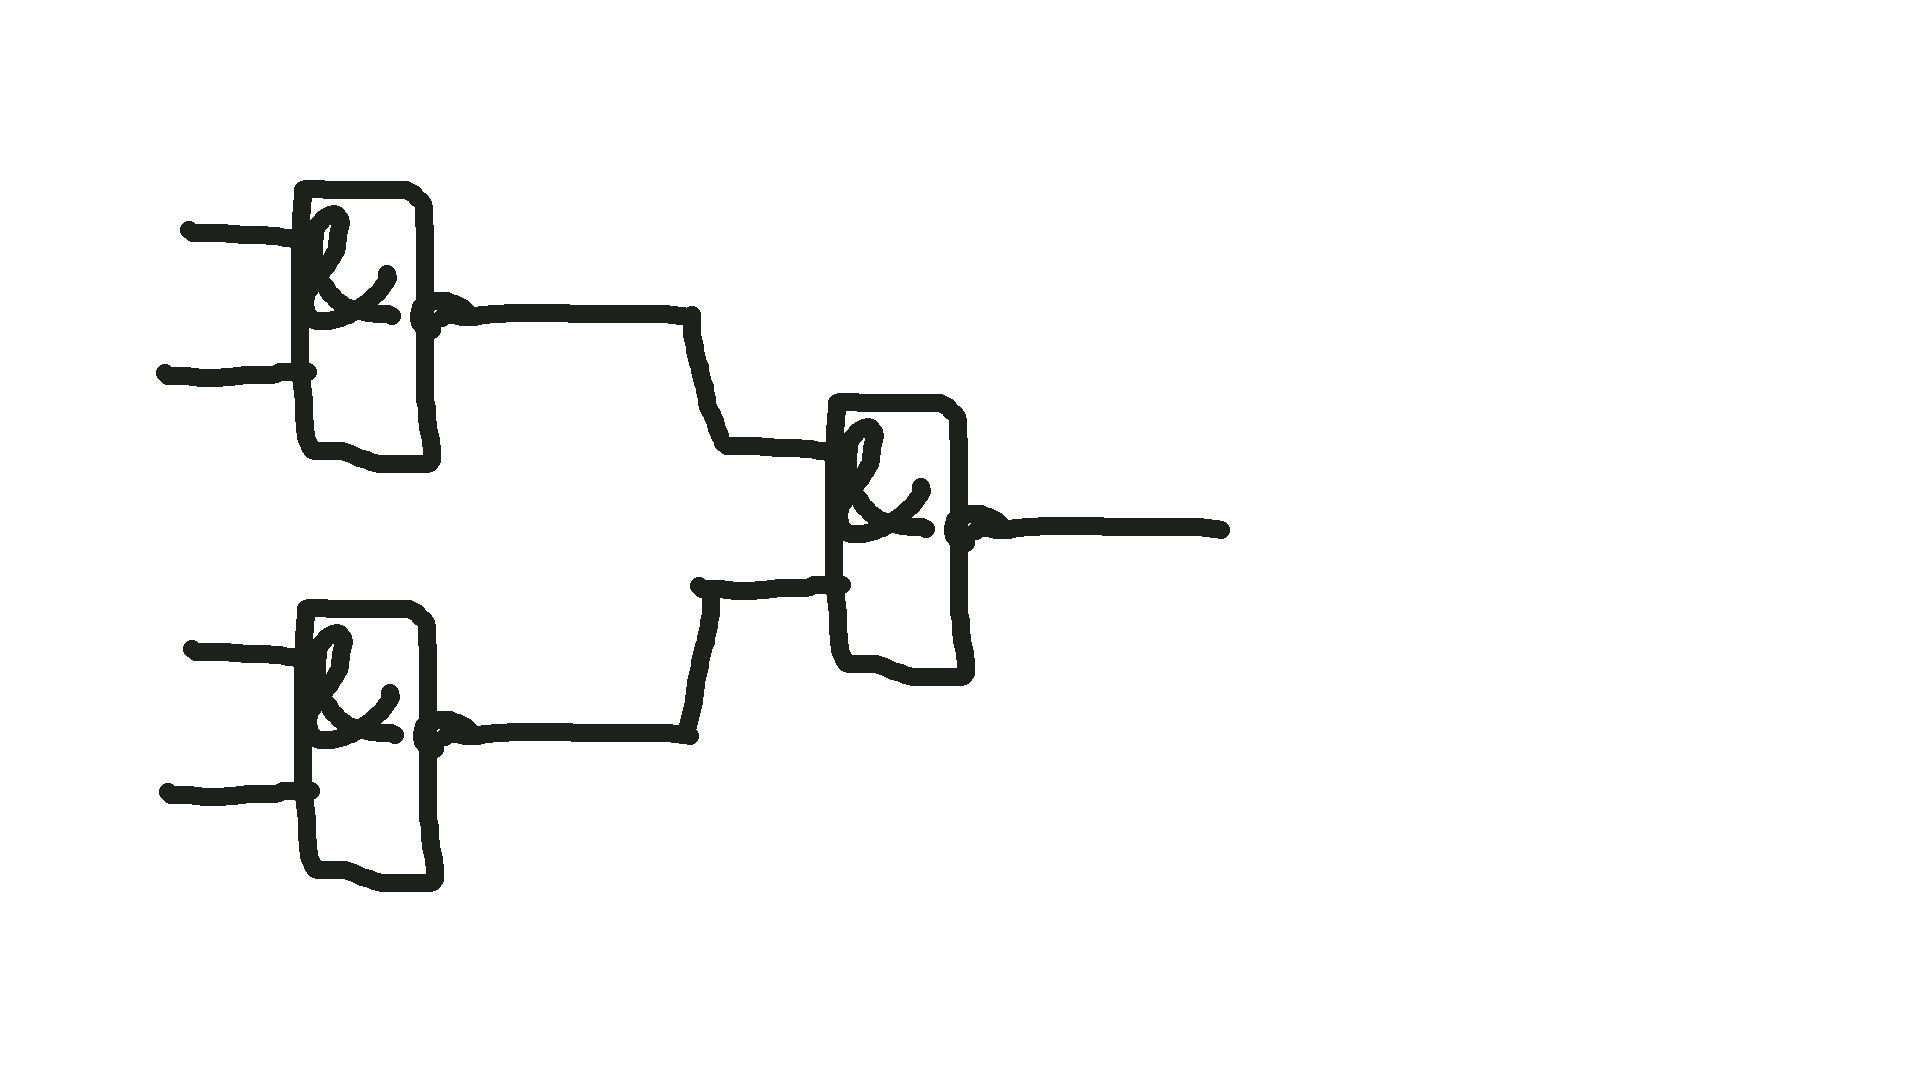
\includegraphics[width=0.85\linewidth]{imgs/1/or-not_and}
	\end{minipage}
	\begin{minipage}{.45\textwidth}
		\centering
		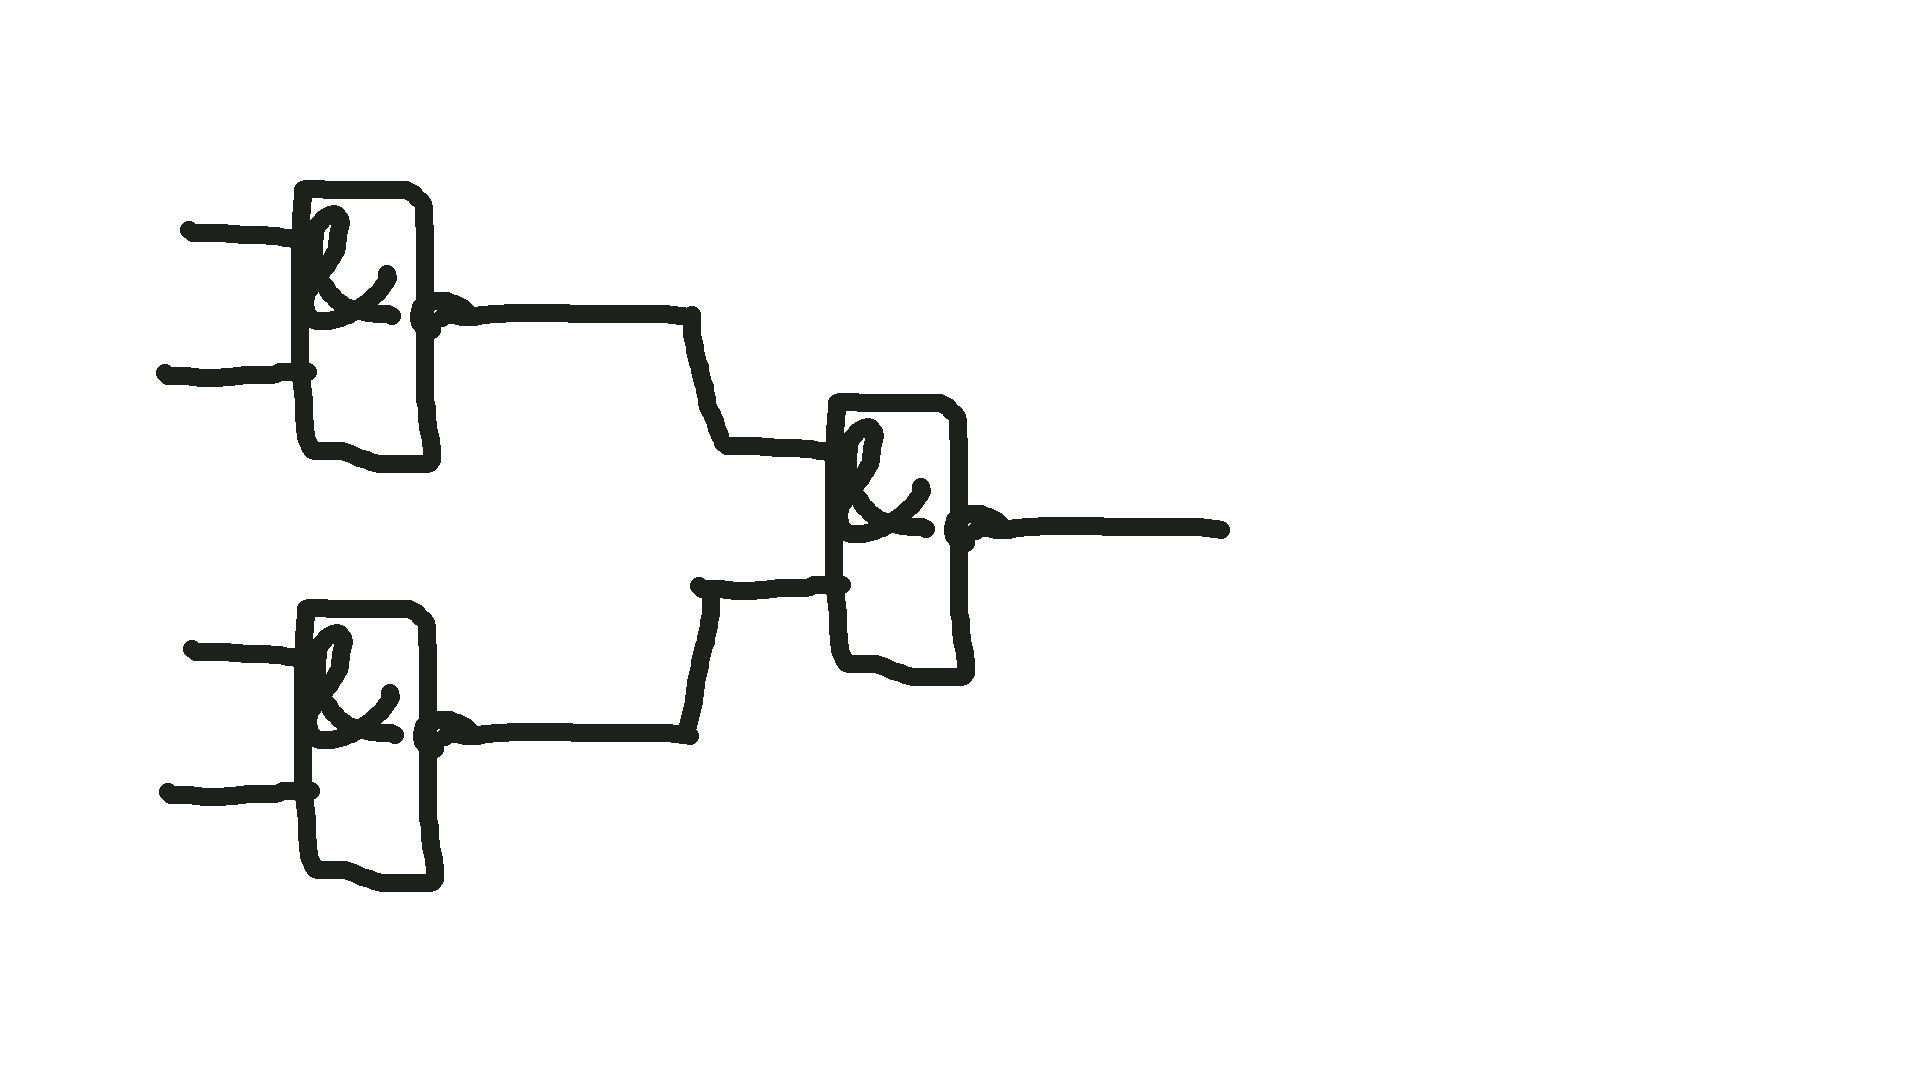
\includegraphics[width=0.85\linewidth]{imgs/1/or-not_or}
	\end{minipage}
	\caption{Реализация элемента ИЛИ-НЕ в базисах 2И-НЕ и 2ИЛИ-НЕ}
\end{figure}

Элемент SN74AHC1G02-EP

Характеристики:
\begin{itemize}
	\item Operating Range from 2 V to 5.5 V
	\item Maximum $t_{pd}$ of 8.5 ns at 5 V
	\item ±8-mA Output Drive at 5 V
\end{itemize}

\subsection{Элемент Искл.ИЛИ}

\begin{figure}[H]
	\centering
	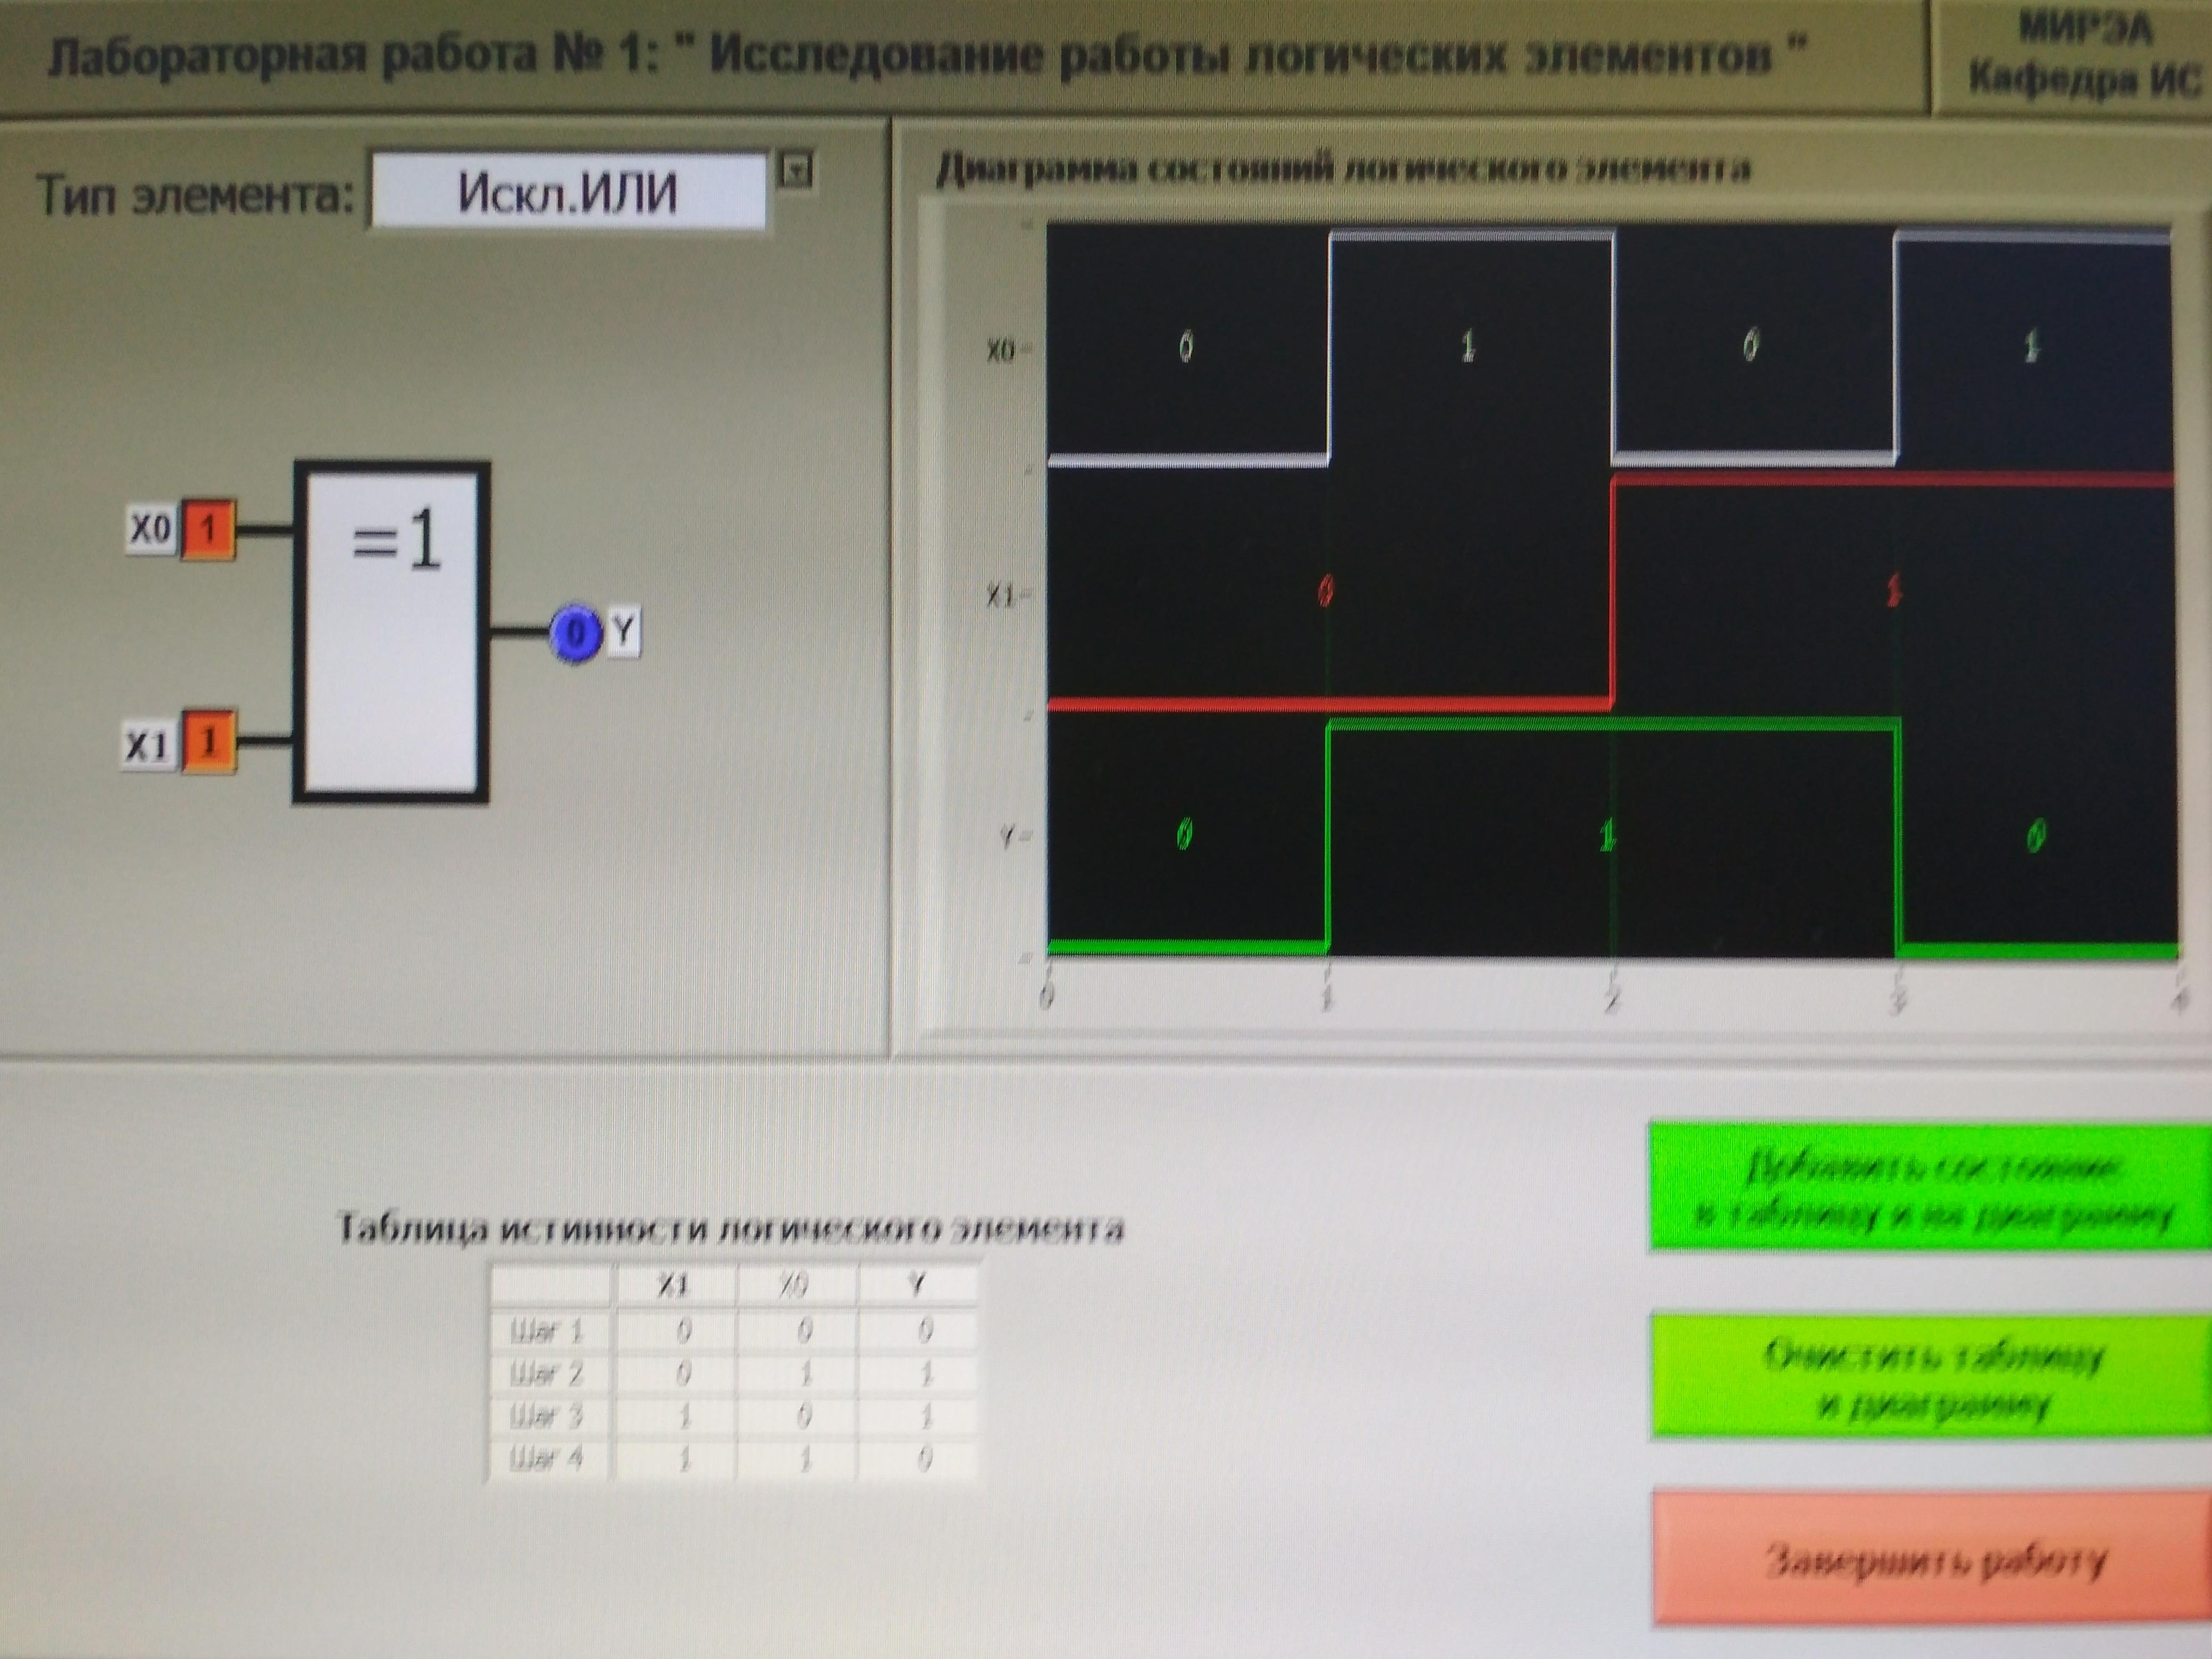
\includegraphics[width=0.85\linewidth]{imgs/1/xor}
	\caption{Результат схемы Искл.ИЛИ}
	\label{fig:1_xor}
\end{figure}

\begin{figure}[H]
	\centering
	\begin{minipage}{.45\textwidth}
		\centering
		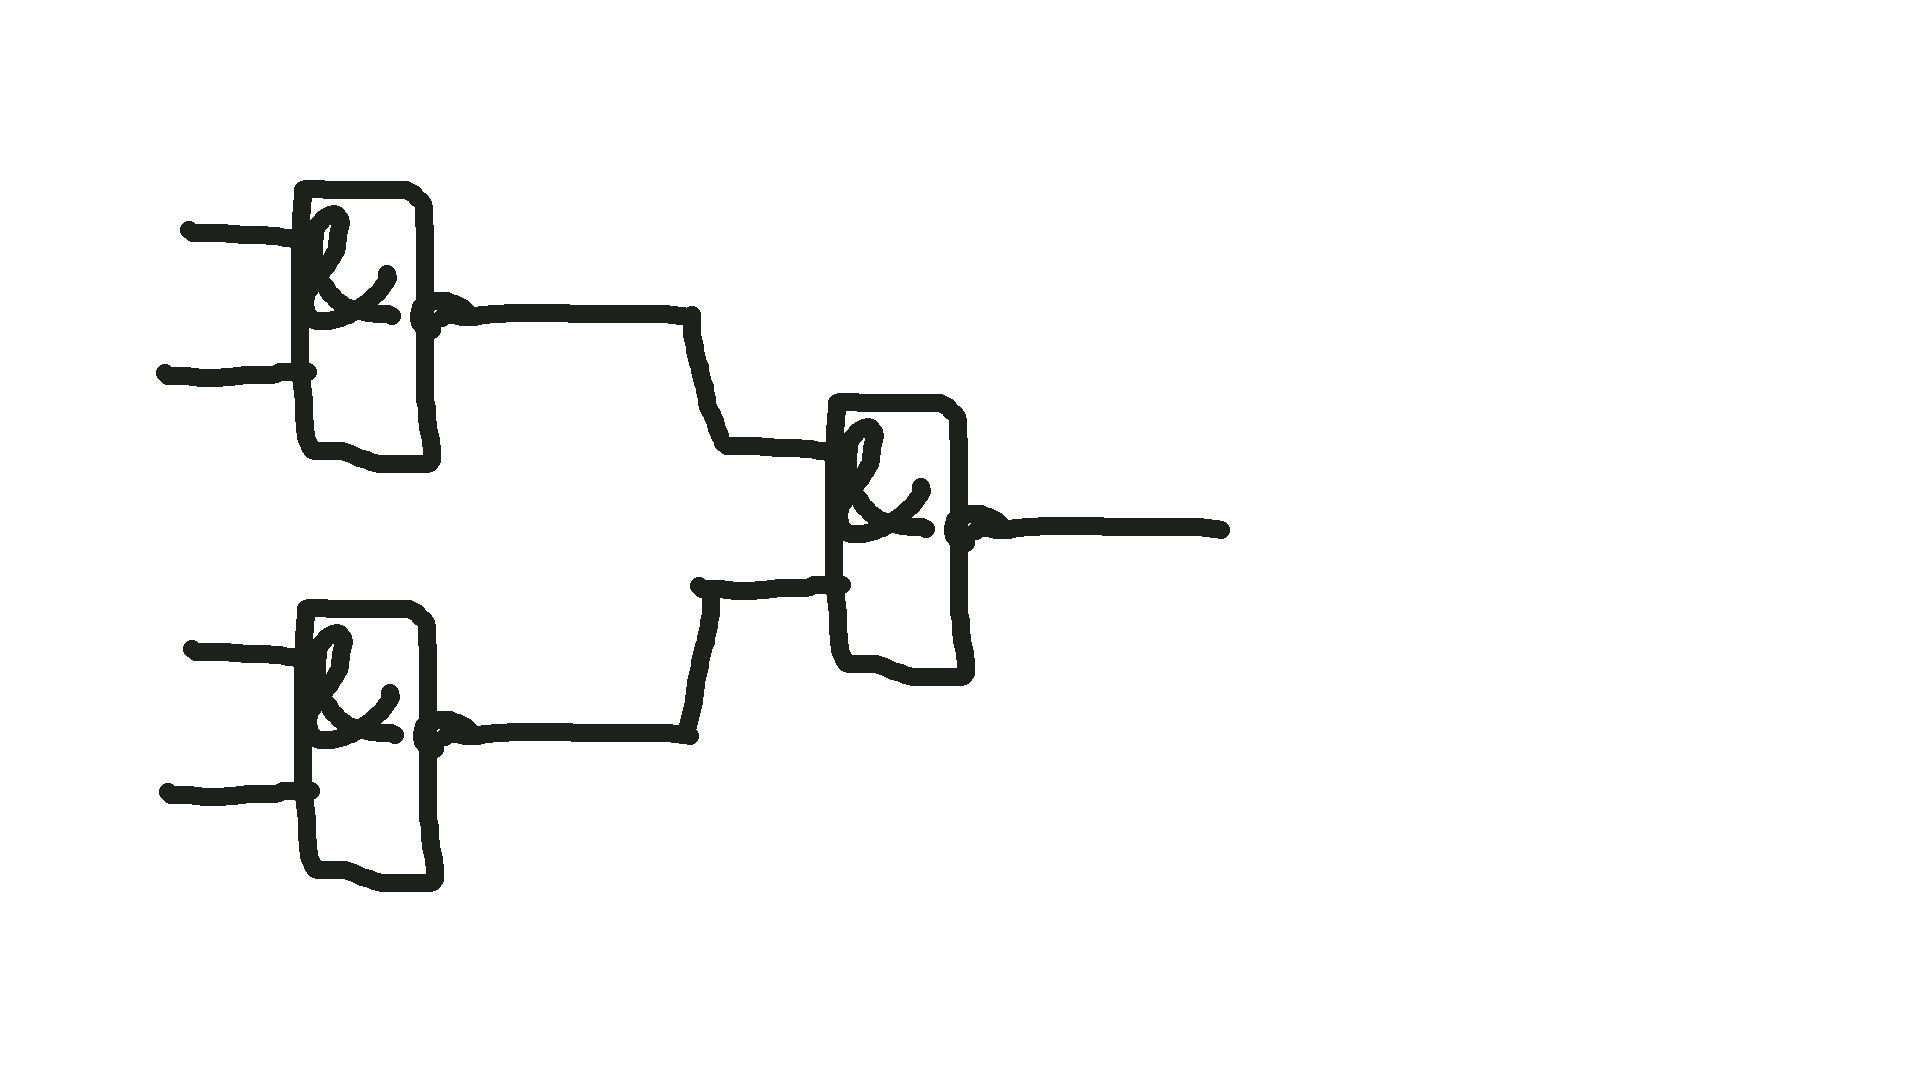
\includegraphics[width=0.85\linewidth]{imgs/1/xor_and}
	\end{minipage}
	\begin{minipage}{.45\textwidth}
		\centering
		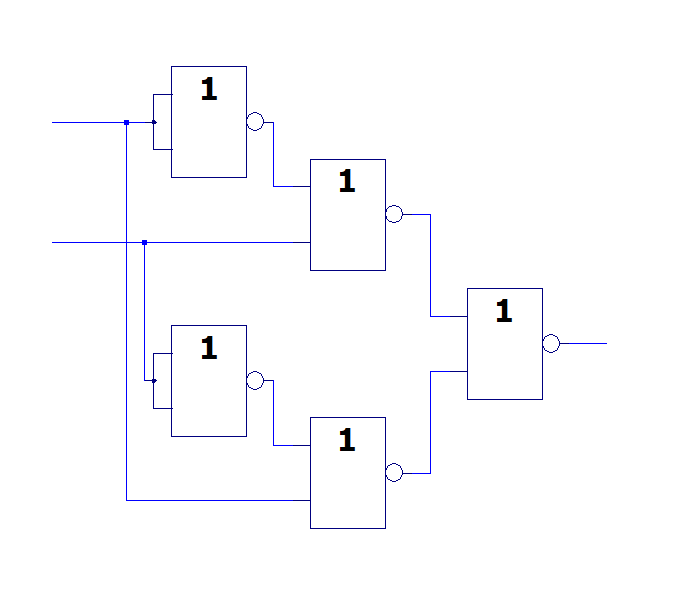
\includegraphics[width=0.85\linewidth]{imgs/1/xor_or}
	\end{minipage}
	\caption{Реализация элемента Искл.ИЛИ в базисах 2И-НЕ и 2ИЛИ-НЕ}
\end{figure}


Элемент SN74LVC1G86-Q1

Характеристики:
\begin{itemize}
	\item Inputs up to 5.5 V
	\item Maximum $t_{pd}$ of 6 ns at 3.3 V
	\item ±24-mA Output Drive at 3.3 V
\end{itemize}